\documentclass{beamer}

\usetheme{Warsaw}

\usepackage[english]{babel}
\usepackage[utf8]{inputenc}
\usepackage{times}
\usepackage[T1]{fontenc}
\usepackage{xcolor}

\title[The CITA on CHIP Project]{The Development of Purdue's Computerized Interactive Teaching Assistant}
\subtitle{Cyrus Vandrevala, Lynn Bryan, Andrew Hirsch, Hisao Nakanishi, Laura Pyrak-Nolte}
\date{August 7, 2015}

\begin{document}

\begin{frame}
  \titlepage
\end{frame}

\begin{frame}
  \tableofcontents
\end{frame}

\section{Introduction}

%%%%%%%%%%%%
% The Need for CITA %
%%%%%%%%%%%%
\subsection*{The Need for CITA}

\begin{frame}{Challenges in Electricity and Optics}
There are many challenges facing us in introductory physics...
\vspace{5mm}
  \begin{itemize}
    \item Increased Enrollment in Online Courses
    \item Weekly Assignments Require Time and Energy
    \item Restricted Access to Teaching Faculty
    \item Non-Traditional Students
  \end{itemize}
\end{frame}

\begin{frame}{Enrollment in Electricity and Optics}
  \begin{figure}
    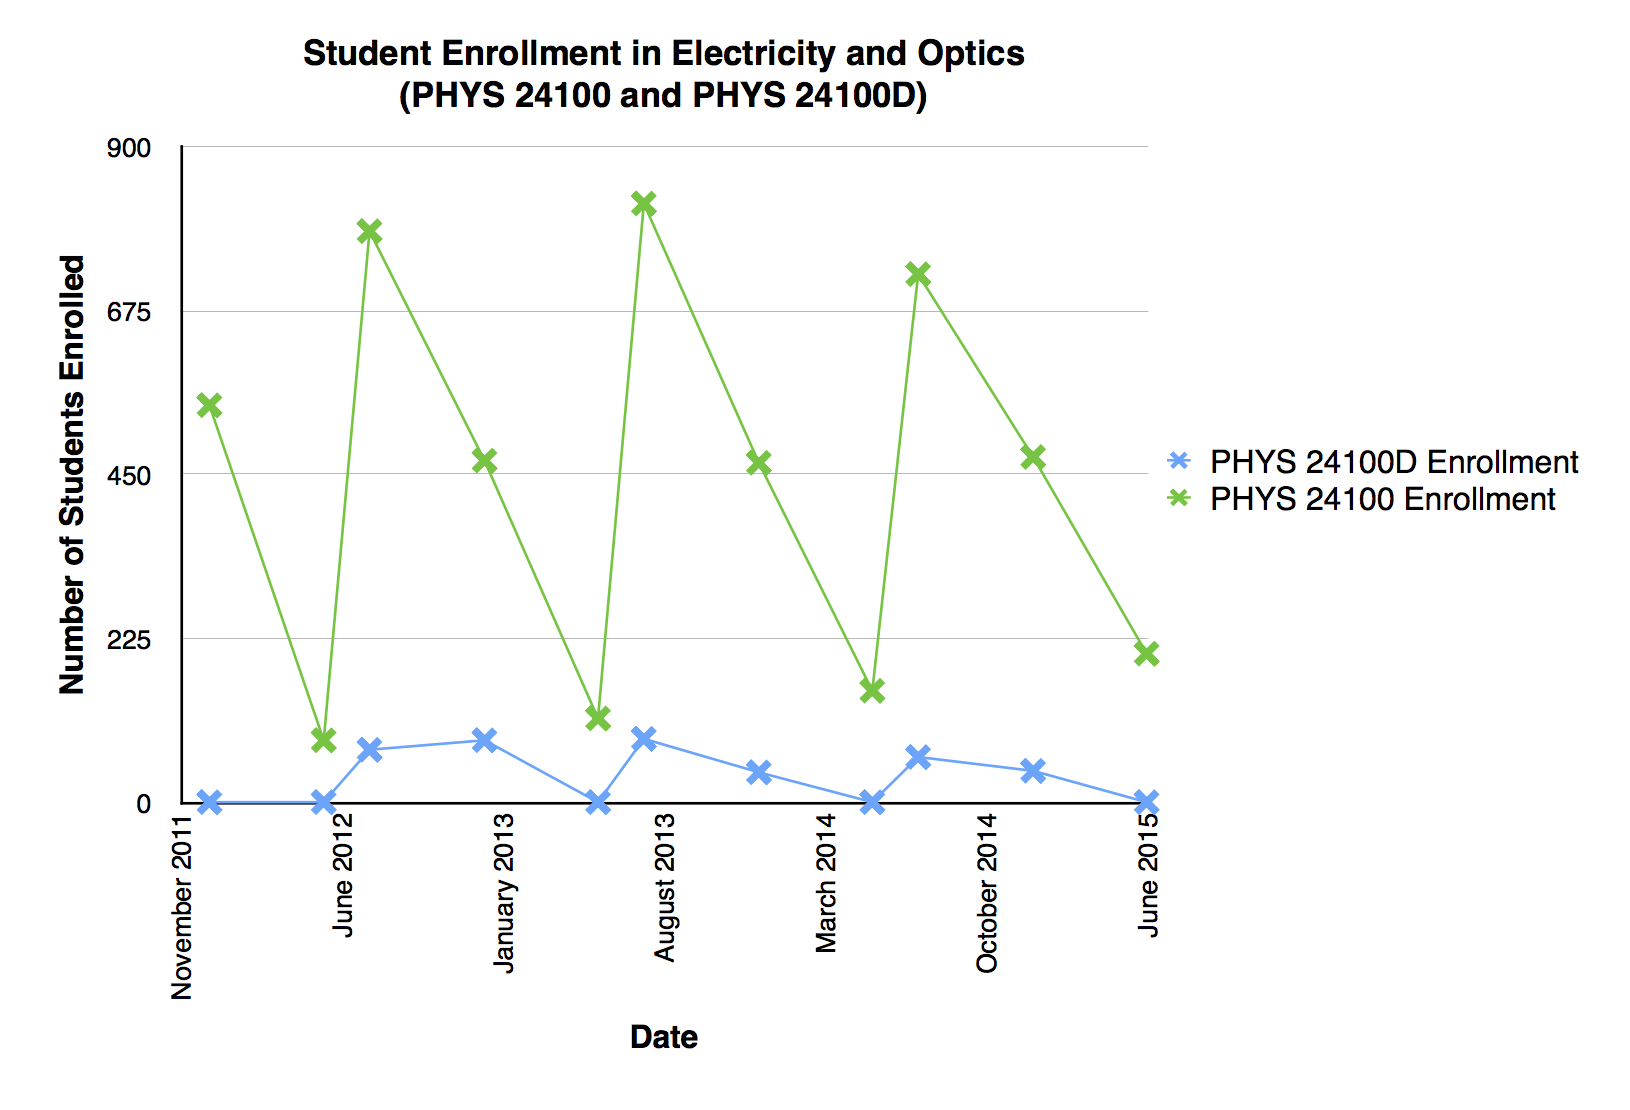
\includegraphics[width=4in]{img/chapter1/enrollment}
  \end{figure}
\end{frame}

\begin{frame}{Broader Challenges in Education}
\begin{center}
The NSF has stated that the knowledge of how to solve complex, real-world problems and create structured experiments is the most important thing that students should learn in their educational careers.
\vspace{5mm}

However, students often do not have these skills when they start their college careers or even after they earn their degree.
\end{center}
\end{frame}

\begin{frame}{Student Opinions}
\begin{quote}
There should be more helping tools, rather than just completing homework. We should have exams relevant to the homework, or reviews/practice of what to expect.
\end{quote}
- Anonymous Student, End of the Semester Evaluation from Fall 2013
\end{frame}

\begin{frame}{Student Opinions}
\begin{quote}
Having a concept map connecting laws and necessary concepts to each other would be helpful as a resource to students. It's difficult enough trying to see connections as learning, but having concept maps that professors/TAs refer back to will allow the students to build with that knowledge in mind.
\end{quote}
- Anonymous Student, End of the Semester Evaluation from Summer 2014
\end{frame}

\begin{frame}{Student Opinions}
\begin{quote}
Thank you for the help section in this problem! It was very well written and helped me figure out the problem and (hopefully) similar ones in the future!
\end{quote}
- Anonymous Student, CHIP Error Report from Fall 2014
\end{frame}

%%%%%%%%%%%%%%%%
% Statement of Development %
%%%%%%%%%%%%%%%%
\subsection*{Statement of Development}

\begin{frame}{Current Tutorials in Introductory Physics}
\begin{columns}
  \begin{column}{2in}
    \begin{figure}
    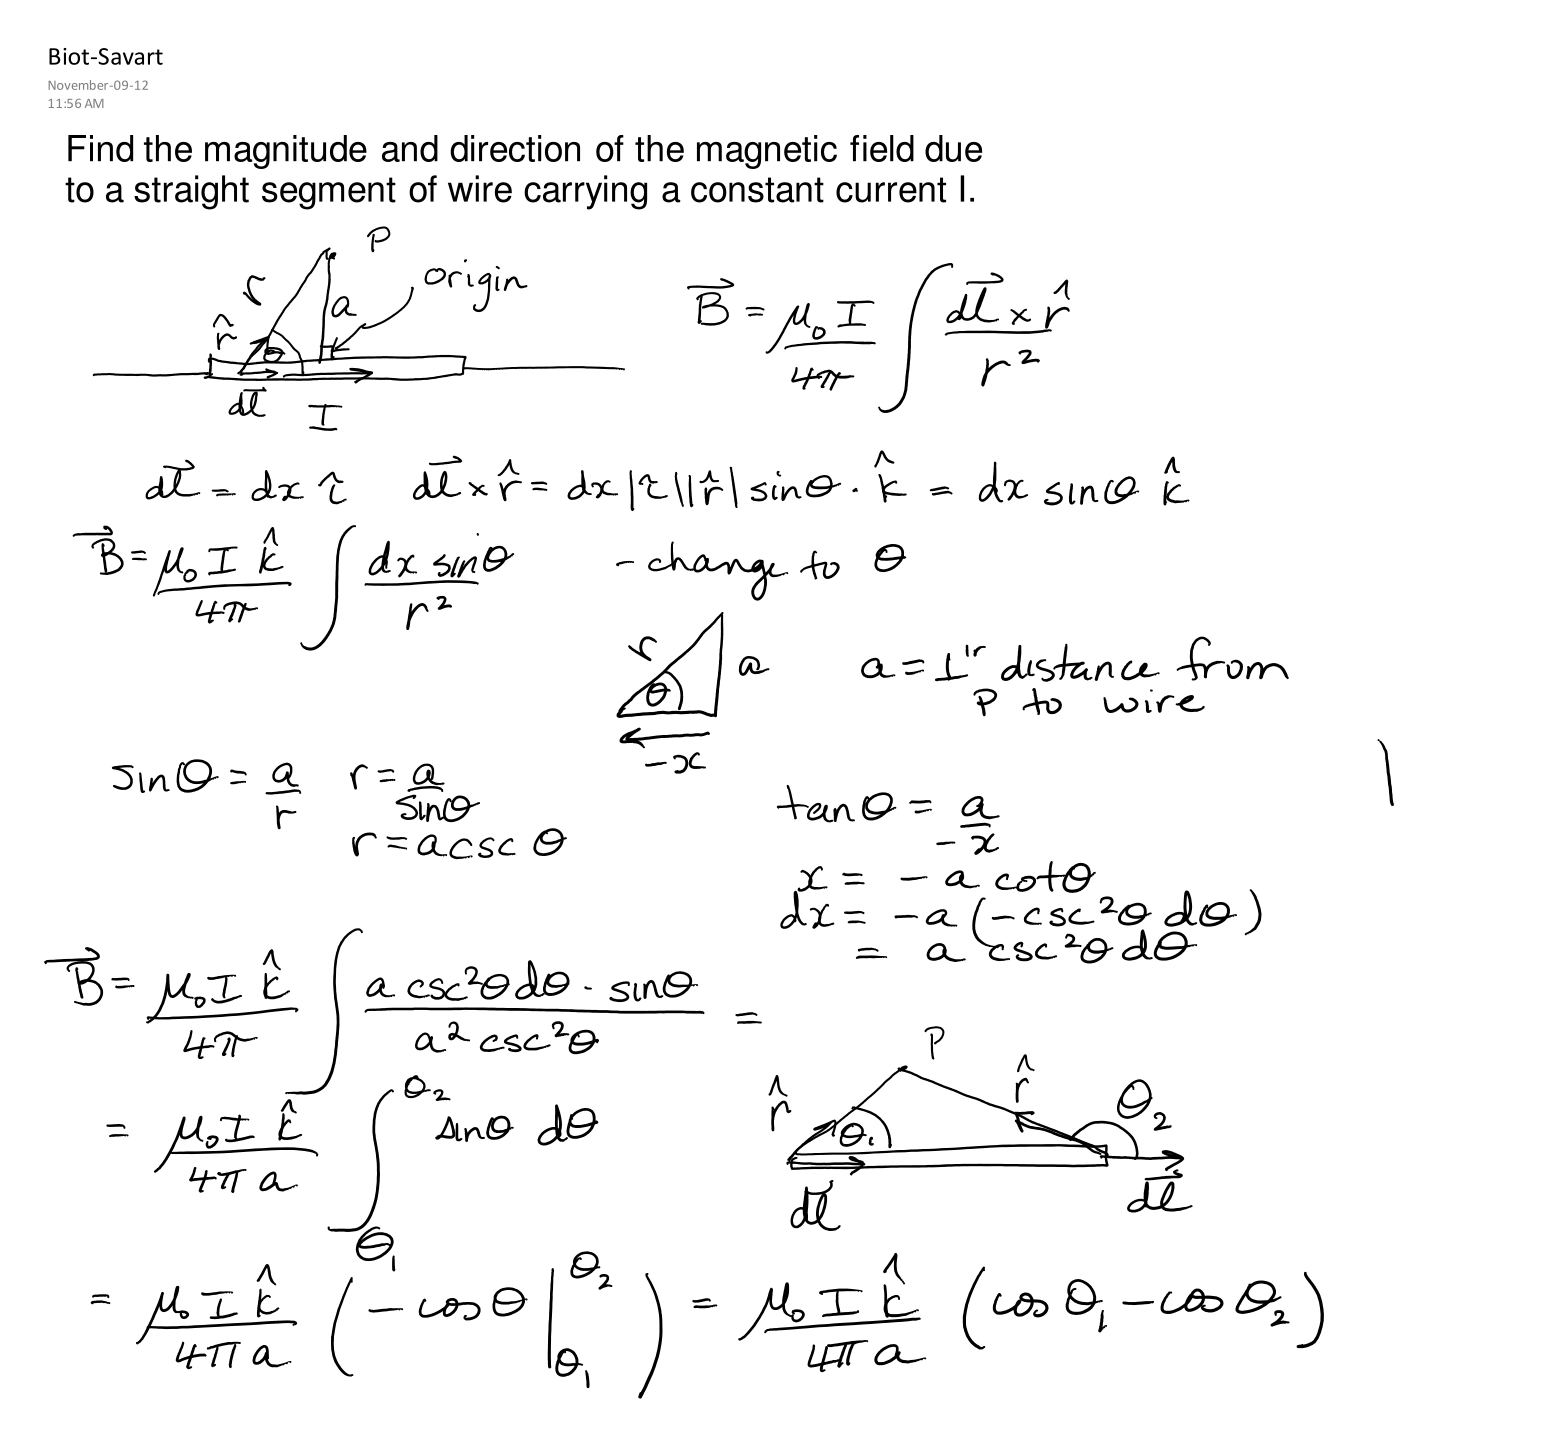
\includegraphics[width=2in]{img/presentation/biot-savart}
  \end{figure}
  \end{column}
  \begin{column}{2in}
  \begin{itemize}
    \item Only a correct/incorrect response to an answer
    \item Little to no explanation as to why the logic of a step of analysis was flawed
    \item Links to notes or the textbook
  \end{itemize}
  \end{column}
  \end{columns}
\end{frame}

\begin{frame}{Statement of Development}
Our goal is to design, develop, implement, and analyze an online system that is available at any time to provide focused guidance to help students acquire the knowledge and skills necessary to solve physics problems.
\vspace{5mm}

The Computerized Interactive Teaching Assistant (CITA) will use a non-linear (branching) structure to guide students through homework problems. This will allow students to explore the concepts in each homework problem in a meaningful way.
\end{frame}

%%%%%%%%%%%%%
% Research Statement %
%%%%%%%%%%%%%
\subsection*{Research Questions}

\begin{frame}{Research Questions}
  \begin{itemize}
  \item How does the branching structure of our interactive tutorials influence student learning of physics concepts?
  \item How does the branching structure of our interactive tutorials influence student problem solving approaches?
  \item What are students perceptions about the CITA system?
  \end{itemize}
\end{frame}

\section{Theoretical Background}

%%%%%%%%%%
% Constructivism %
%%%%%%%%%%
\subsection*{Constructivism}

\begin{frame}{The Learning Philosophy of Constructivism}
\begin{itemize}
\item Knowledge is not something that is passively received.
\item Knowledge is actively built up over time through experience.
\item This adaptive knowledge is meant to organize the world.
\item An organized worldview is not necessarily a correct worldview.
\end{itemize}
\end{frame}

\begin{frame}{Constructivism in Physics}
  \begin{figure}
  \centering
    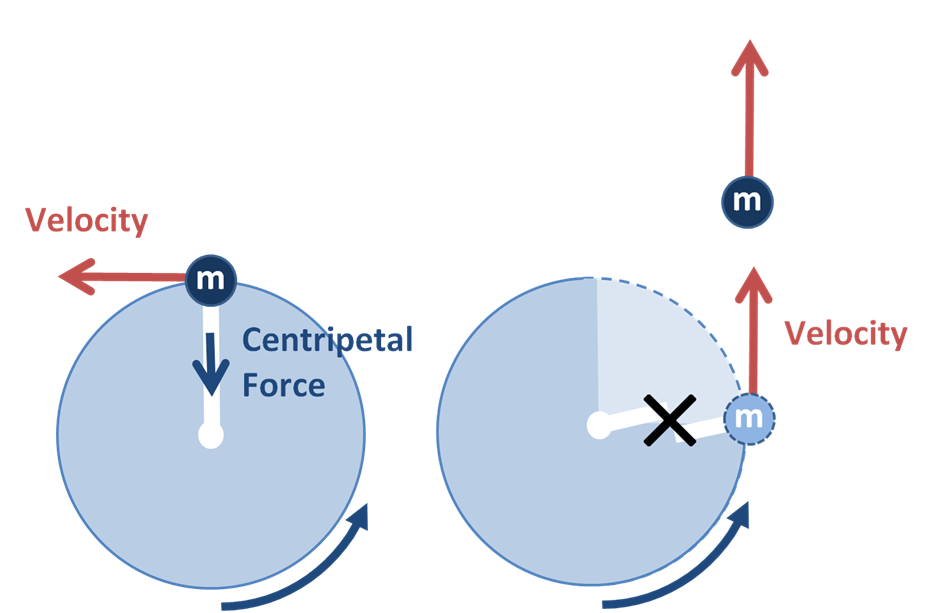
\includegraphics[width=2.5in]{img/presentation/ucm_string}
    \caption{Courtesy of Wikimedia.}
  \end{figure}
\end{frame}

\begin{frame}{Constructivism in Physics}
  \begin{figure}
  \centering
    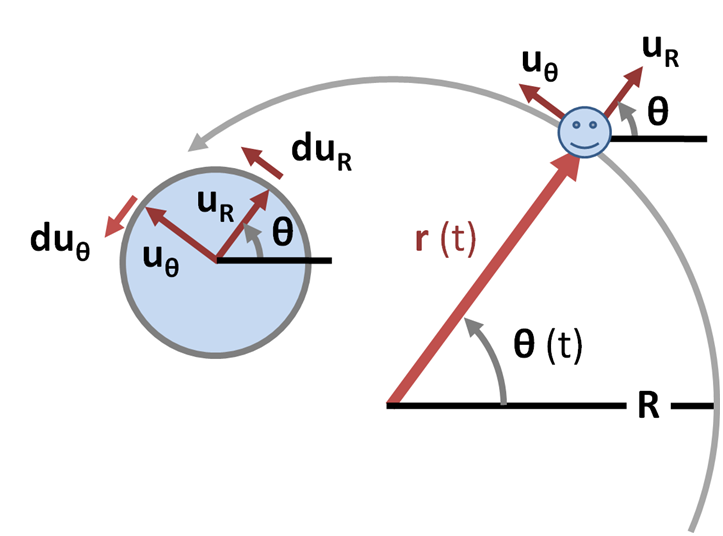
\includegraphics[width=2.5in]{img/presentation/vectors}
    \caption{Courtesy of Wikimedia.}
  \end{figure}
\end{frame}

%%%%%%%%%%%
% Problem Solving %
%%%%%%%%%%%
\subsection*{Problem Solving}

\begin{frame}{Polya's Strategy for Problem Solving}
The modern theory of problem solving is rooted in the work of George Polya. He outlined a deceptively simple strategy for solving a problem:
\vspace{5mm}
\begin{enumerate}
\item Understand the Problem
\item Devise a Plan
\item Execute the Plan
\end{enumerate}
\end{frame}

\begin{frame}{Problem Solving in Physics}
Most people cannot get through those three steps!
\vspace{5mm}
\begin{itemize}
\item Expert vs. Novice
\item First Principles vs. Searching
\item Forwards vs. Backwards
\end{itemize}
\end{frame}

%%%%%%%%
% Scaffolding %
%%%%%%%%
\subsection*{Scaffolding}

\begin{frame}{Scaffolding in Childhood Development}
The method of scaffolding is based on the work of Lev Vygotsky.
  \begin{figure}
  \centering
    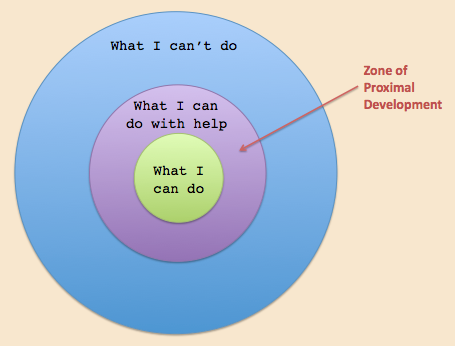
\includegraphics[width=2in]{img/presentation/zpd}
    \caption{Courtesy of Innovative Learning.}
  \end{figure}
\end{frame}

\begin{frame}{Scaffolding in the Classroom}
Back to the diagram from earlier...
\vspace{5mm}
  \begin{figure}
  \centering
    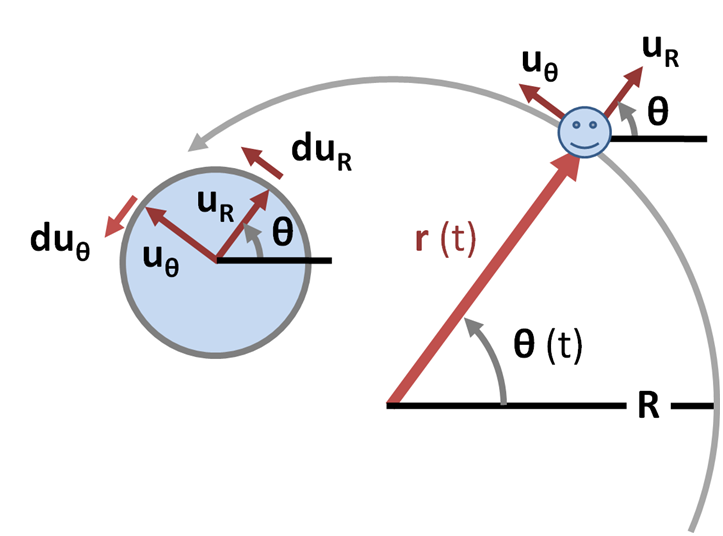
\includegraphics[width=2in]{img/presentation/vectors}
    \caption{Courtesy of Wikimedia.}
  \end{figure}
\end{frame}

%%%%%%%%%%%%%%%
% Interactive Engagement %
%%%%%%%%%%%%%%%
\subsection*{Interactive Engagement}

\begin{frame}{Interactive Engagement Methods}
\begin{itemize}
\item Interactive engagement methods challenge students to think about concepts in a deeper, more meaningful way.
\item They frown upon generic problems that can be solved in one or two steps - so called ``plug and chug'' problems. 
\item They stress classroom interactions and real-world analysis.
\end{itemize}
\end{frame}

\begin{frame}{Interactive Engagement Methods}
\begin{itemize}
\item Just-in-Time Teaching
\item Activity Based Physics
\item Workshop Physics
\item Socratic Dialogue Inducing Methods
\item Peer Instruction
\item And Many More...
\end{itemize}
\end{frame}

\section{The CITA System}

\subsection*{Demonstration}

\begin{frame}{Demonstration}
\begin{center}
Let's see the CITA system in action.
\end{center}
\end{frame}

%%%%%%%%%%%%%
% Quantitative Methods %
%%%%%%%%%%%%%
\subsection*{Quantitative Methods}

\begin{frame}{Quantitative Methods}
\begin{itemize}
\item Classroom Artifact Data
\begin{itemize}
\item Homework
\item Quizzes
\item Exams
\end{itemize}
\item BEMA Exam
\item Multi-Step Problem
\item Online Surveys
\begin{itemize}
\item Demographics Survey
\item Student Exit Survey
\end{itemize}
\end{itemize}
\end{frame}

%%%%%%%%%%%%
% Qualitative Methods %
%%%%%%%%%%%%
\subsection*{Qualitative Methods}

\begin{frame}{Qualitative Methods}
\begin{itemize}
\item Focus Group Sessions
\item Follow-Up Personal Interviews
\begin{itemize}
\item Optional Sessions Given to Participants from Focus Groups
\end{itemize}
\item Piazza Data
\begin{itemize}
\item Improve CITA Questions
\item Fill in Gaps in Interviews
\end{itemize}
\end{itemize}
\end{frame}

\section{Results}

%%%%%%
% BEMA %
%%%%%%
\subsection*{BEMA}

\begin{frame}{Overview of the BEMA}
\begin{itemize}
\item BEMA is an acronym for the Brief Electricity and Magnetism Assessment.
\item It tests conceptual understanding of electromagnetism topics.
\item We administered the BEMA in the spring and summer semesters of 2015.
\end{itemize}
\end{frame}

\begin{frame}{Spring vs. Summer 2015}
\begin{columns}
\begin{column}{2in}
\begin{figure}
	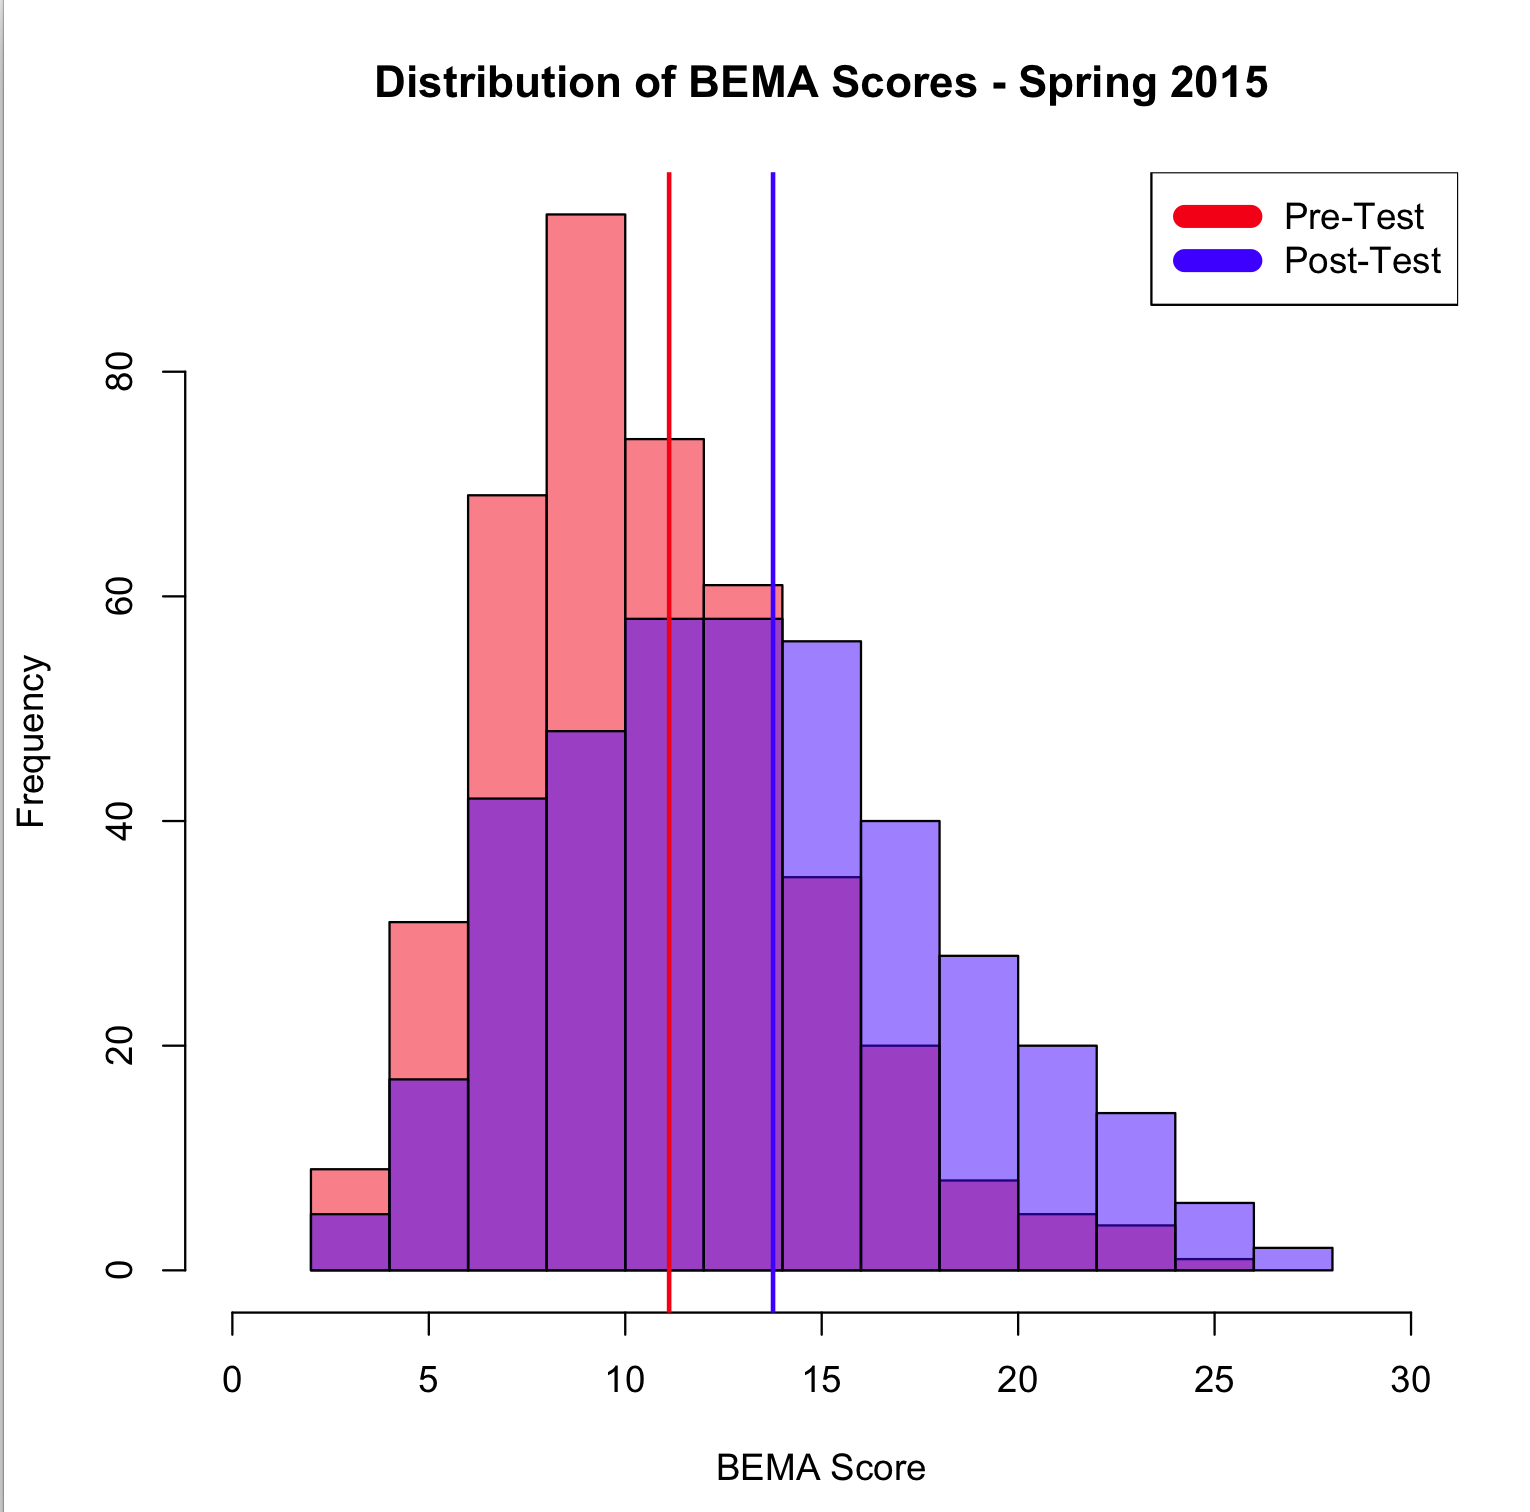
\includegraphics[width=2in]{img/chapter4/bema_spring_2015}
\end{figure}
\end{column}
\begin{column}{2in}
\begin{figure}
	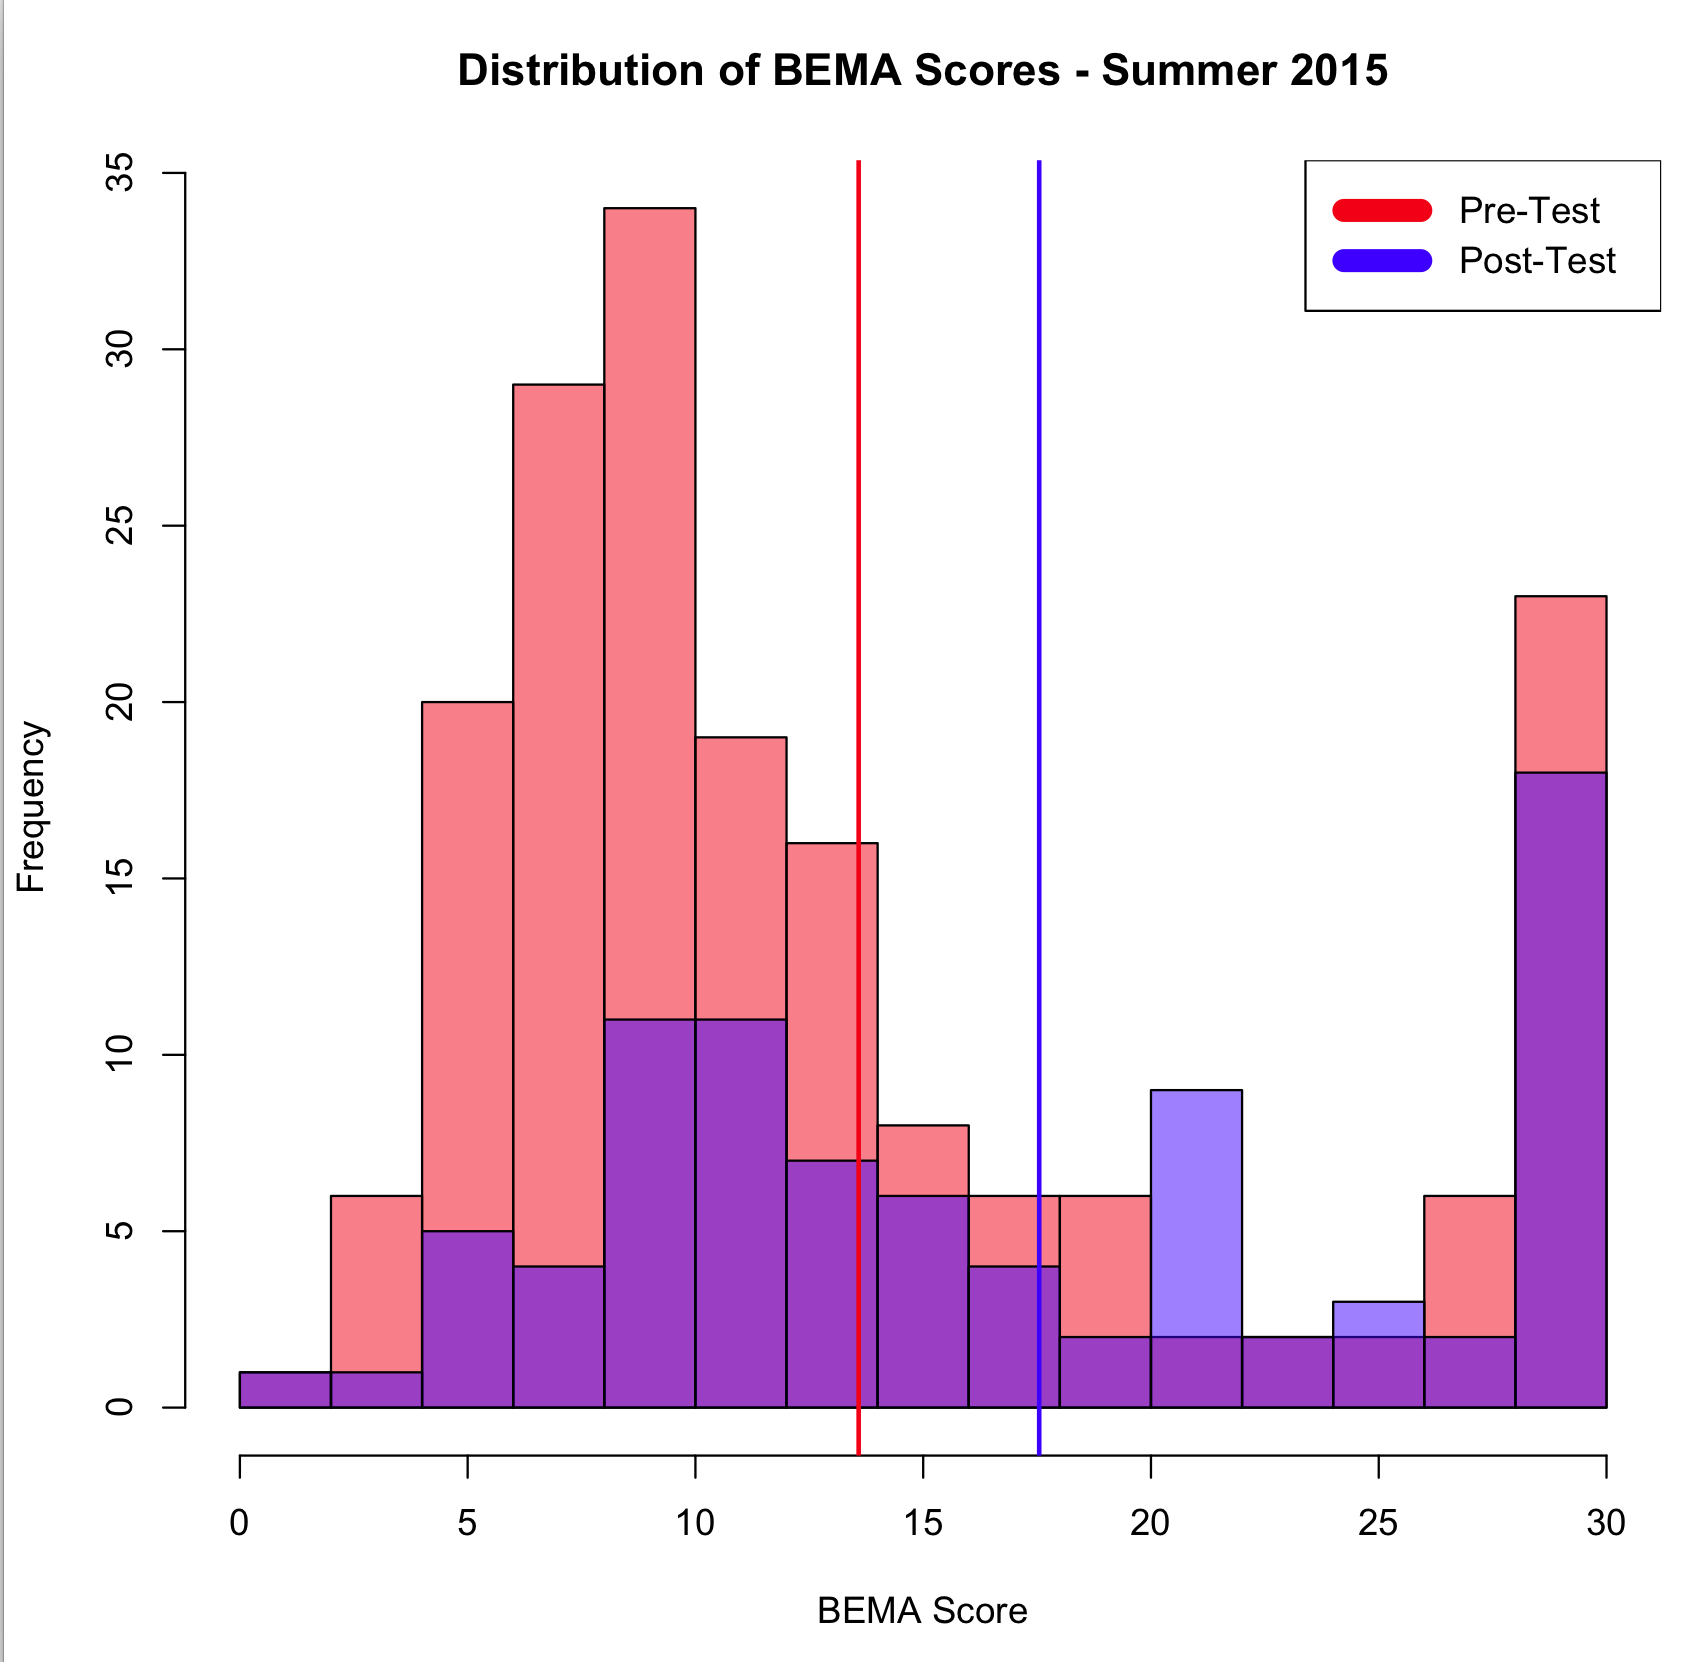
\includegraphics[width=2in]{img/chapter4/bema_summer_2015}
\end{figure}
\end{column}
\end{columns}
\end{frame}

\begin{frame}{Spring 2015 vs. Summer 2015}
\begin{columns}
\begin{column}{2in}
\begin{figure}
	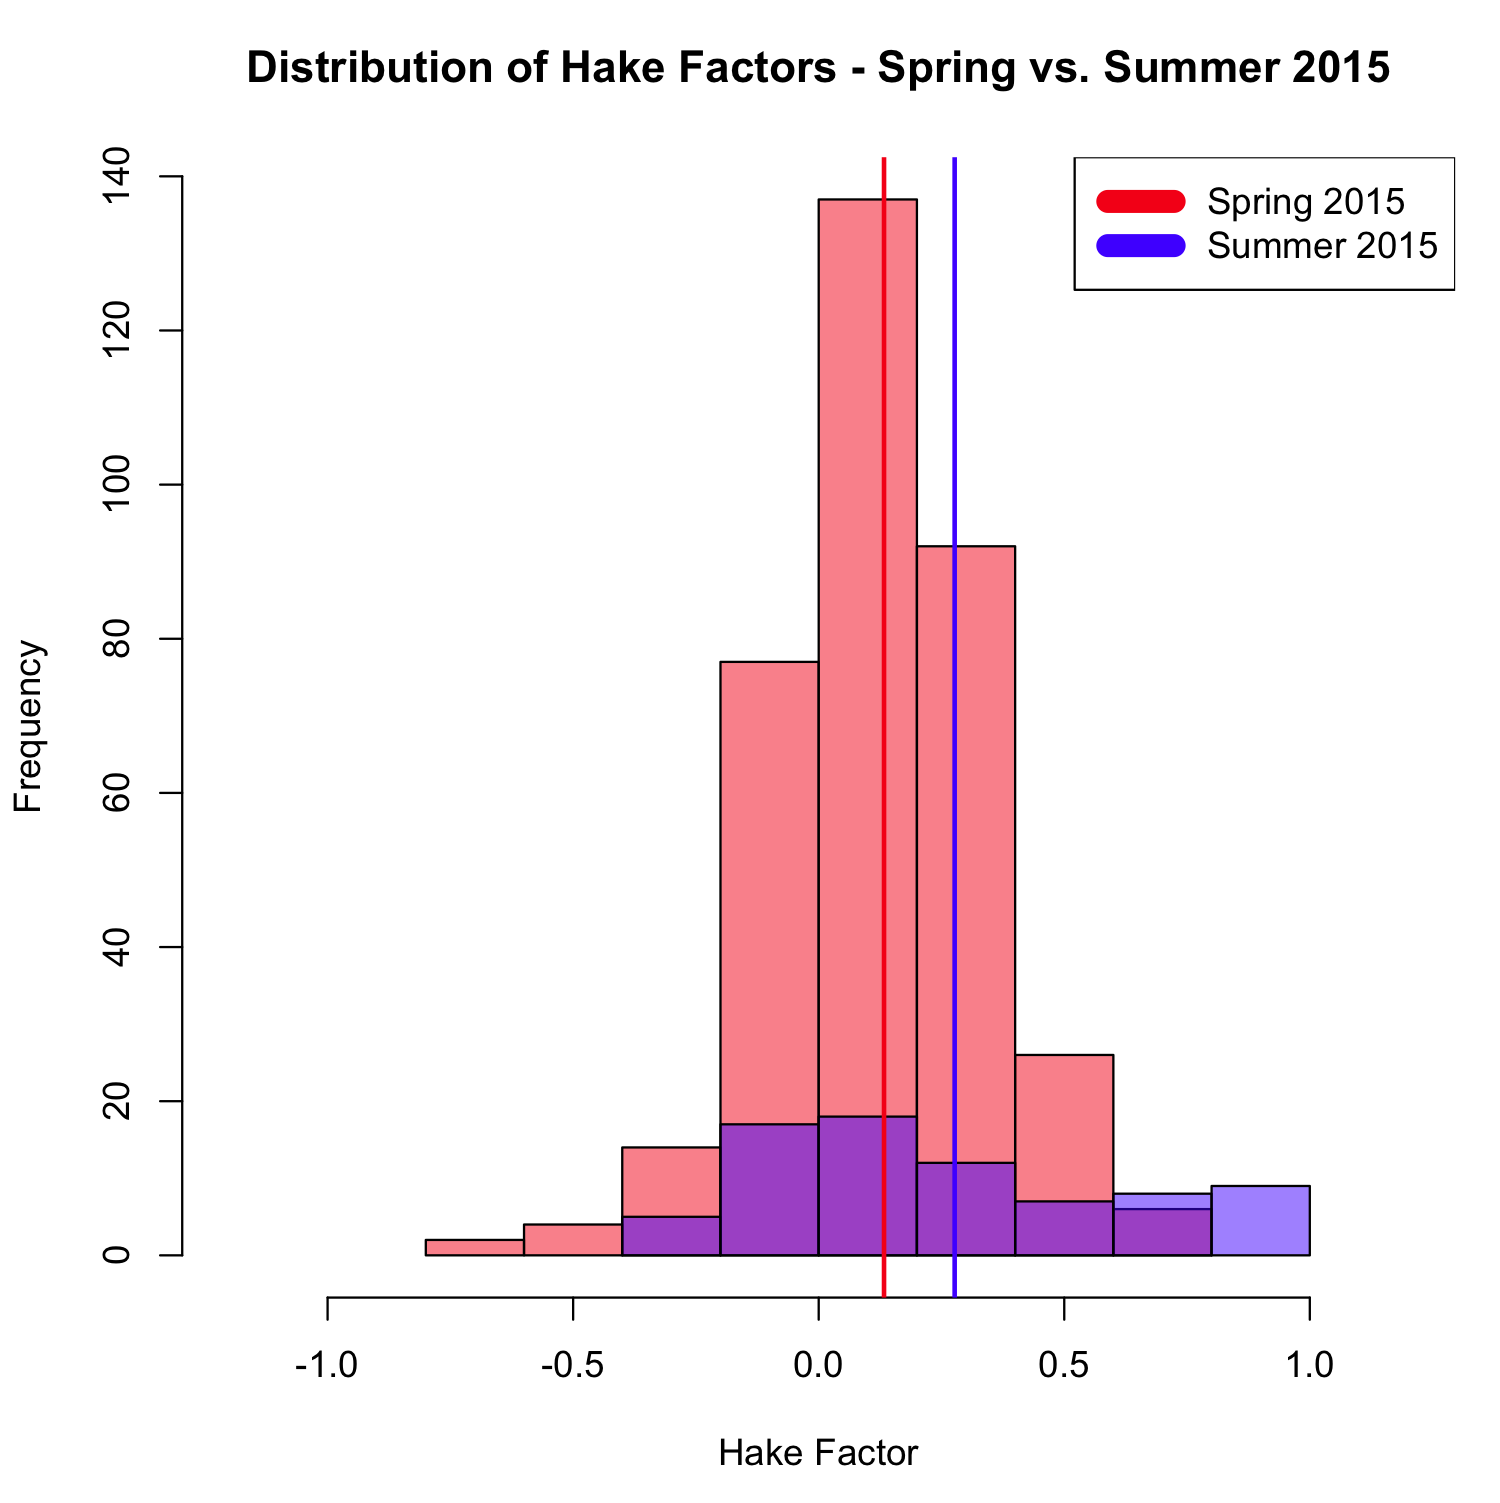
\includegraphics[width=2in]{img/chapter4/hake_spring_vs_summer_filtered}
\end{figure}
\end{column}
\begin{column}{2in}
\begin{scriptsize}
\begin{table}
  \begin{tabular}{|l|l|}
    \hline
    \textbf{Statistic} & \textbf{Value} \\
	\hline
	$\mu$ - Su 2015 & 0.263 \\
	\hline
	$\mu$ - Sp 2015 & 0.133 \\
	\hline
	$\sigma$ - Su 2015 & 0.440 \\
	\hline
	$\sigma$ - Sp 2015 & 0.208 \\
	\hline
	Shapiro-Wilk - Su 2015 & p = 8.509e-06 \\
	\hline
	Shapiro-Wilk - Sp 2015 & p = 6.683e-05 \\
	\hline
	Wilcoxon Signed-Rank & p = 0.009334 \\
	\hline
	Cohen's D & 0.503 \\
	\hline
  \end{tabular}
\end{table}
\end{scriptsize}
\end{column}
\end{columns}
\end{frame}

\begin{frame}{Spring 2015 (Distance Learning) vs. Summer 2015}
\begin{columns}
\begin{column}{2in}
\begin{figure}
	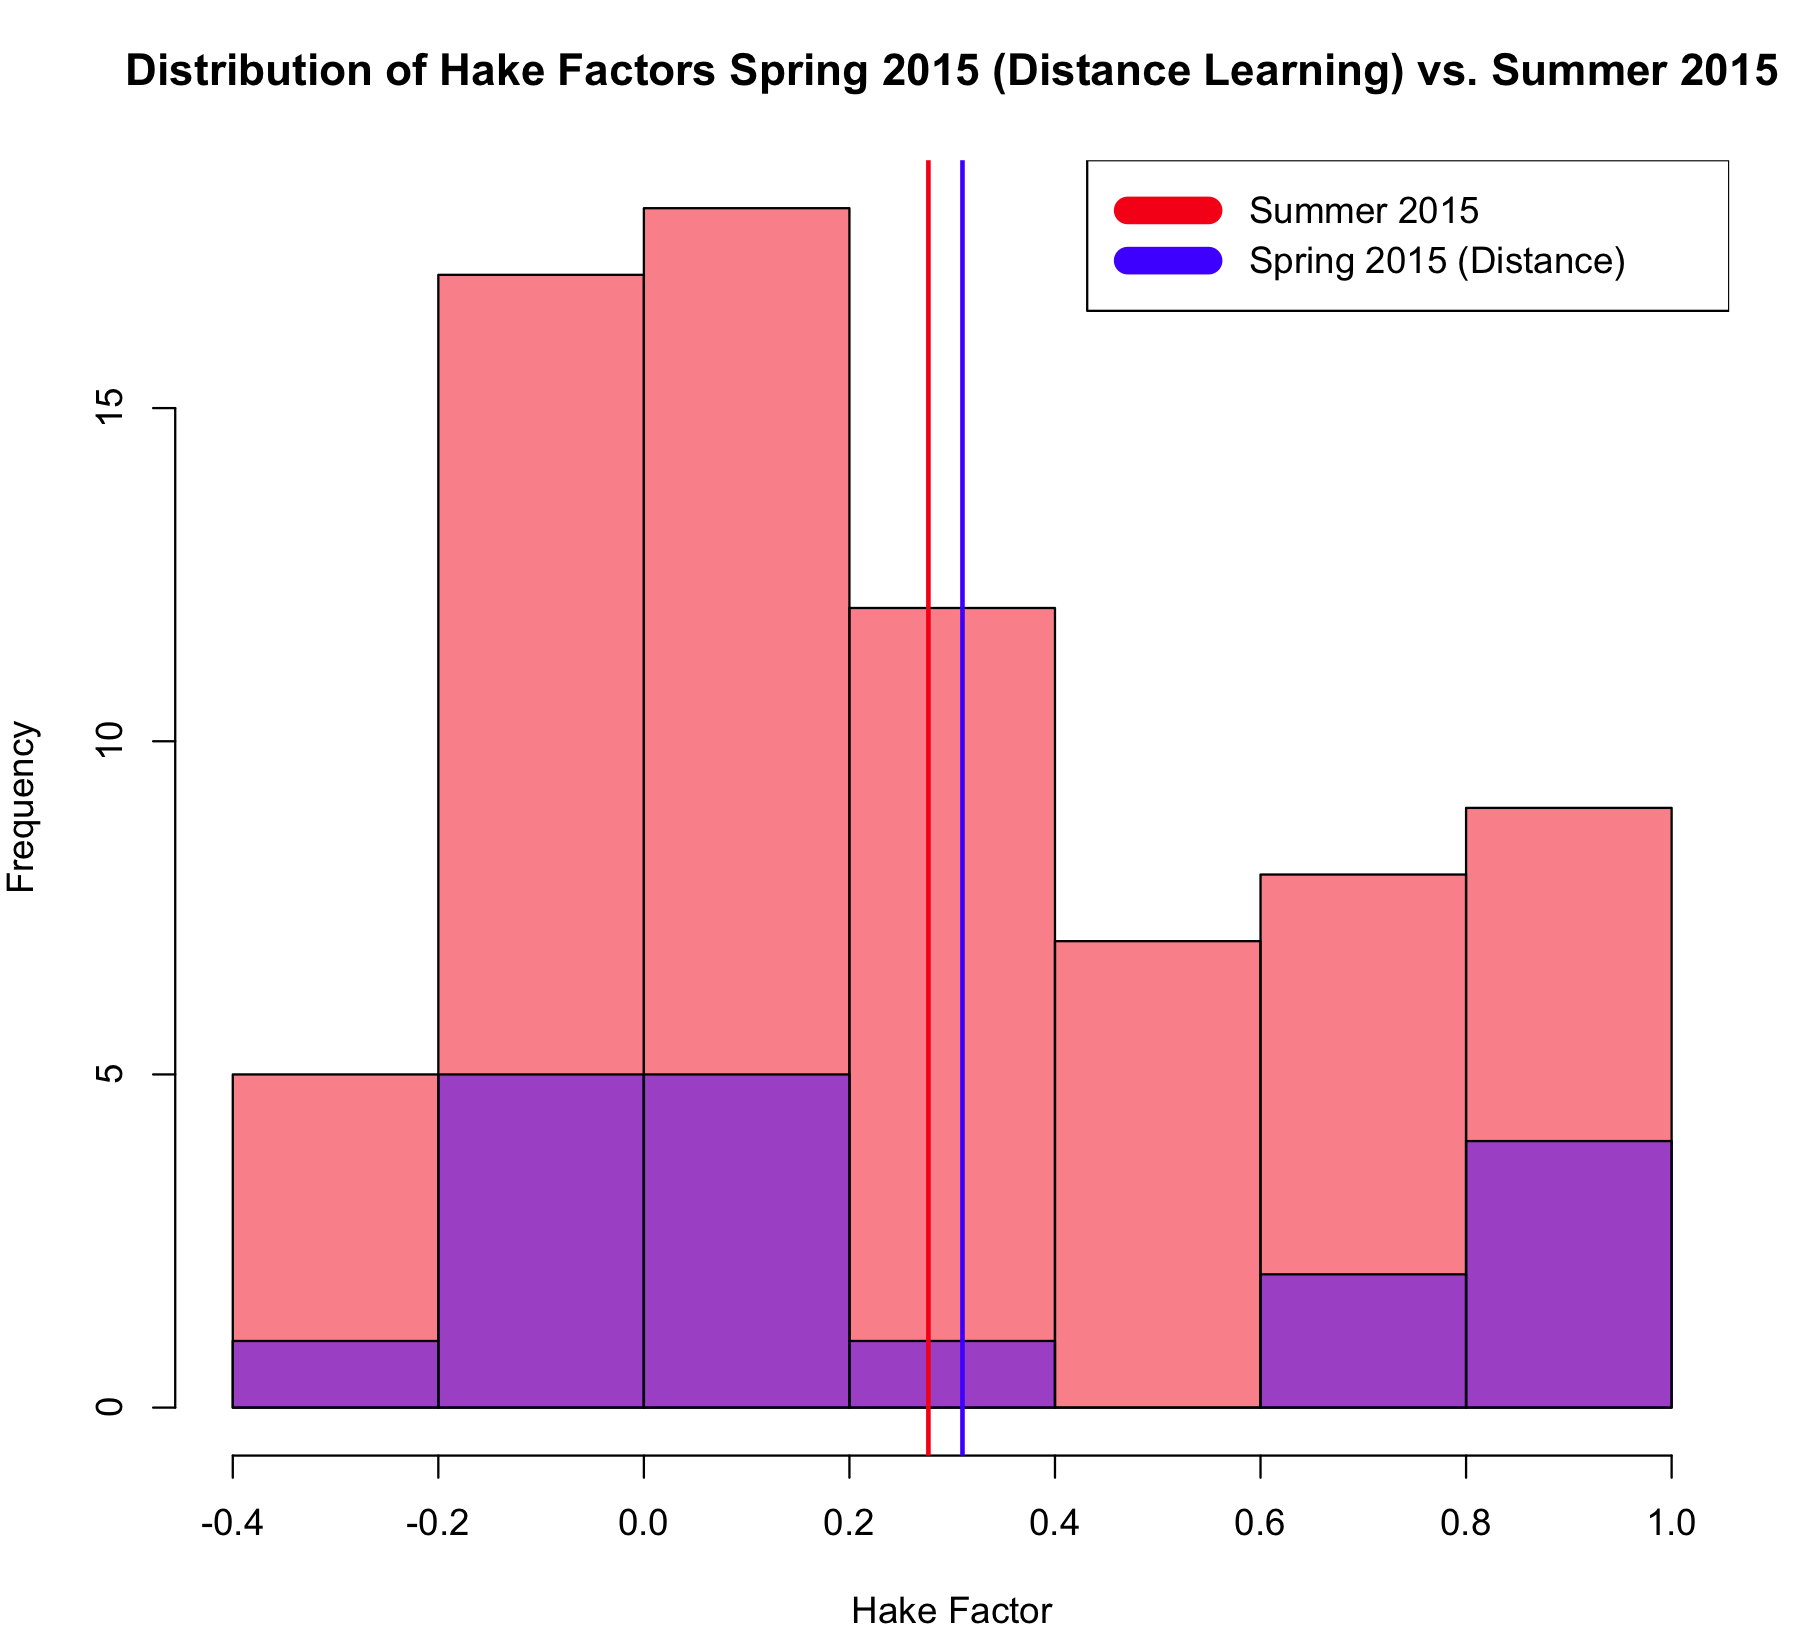
\includegraphics[width=2in]{img/chapter4/hake_su15_vs_sp15d}
\end{figure}
\end{column}
\begin{column}{2in}
\begin{scriptsize}
\begin{table}
  \begin{tabular}{|l|l|}
    \hline
    \textbf{Statistic} & \textbf{Value} \\
	\hline
	$\mu$ - Su 2015 & 0.263 \\
	\hline
	$\mu$ - Sp 2015 & 0.31 \\
	\hline
	$\sigma$ - Su 2015 & 0.440 \\
	\hline
	$\sigma$ - Sp 2015 & 0.426 \\
	\hline
	Shapiro-Wilk - Su 2015 & p = 8.509e-06 \\
	\hline
	Shapiro-Wilk - Sp 2015 & p = 0.009379 \\
	\hline
	Wilcoxon Signed-Rank & p = 0.9028 \\
	\hline
	Cohen's D & 0.107 \\
	\hline
  \end{tabular}
\end{table}
\end{scriptsize}
\end{column}
\end{columns}
\end{frame}

\begin{frame}{Trends with BEMA Scores}
  \begin{itemize}
    \item It is difficult to say for certain which scores can be trusted.
    \item After filtering out some of the scores that demonstrated cheating, we find that there is an increase in the mean of the BEMA scores between summer 2015 and spring 2015.
    \item After filtering out some of the scores that demonstrated cheating, we find that there is no difference in the mean of the BEMA scores between summer 2015 and spring 2015.
  \end{itemize}
\end{frame}

%%%%%%%%
% Homework %
%%%%%%%%
\subsection*{Homework}

\begin{frame}{Overview of CHIP Homework}
  \begin{itemize}
    \item Homework assignments are administered online through CHIP.
    \item Homework assignments are usually due one per week during the spring and fall.
    \item Homework assignments are due two per week during the summer due to the shorter timespan of the summer session.
    \item A full writeup of the scoring policy and submission rules can be found on the CHIP website.
  \end{itemize}
\end{frame}

\begin{frame}{Summer 2014 vs. Summer 2015}
\begin{columns}
\begin{column}{2in}
\begin{figure}
	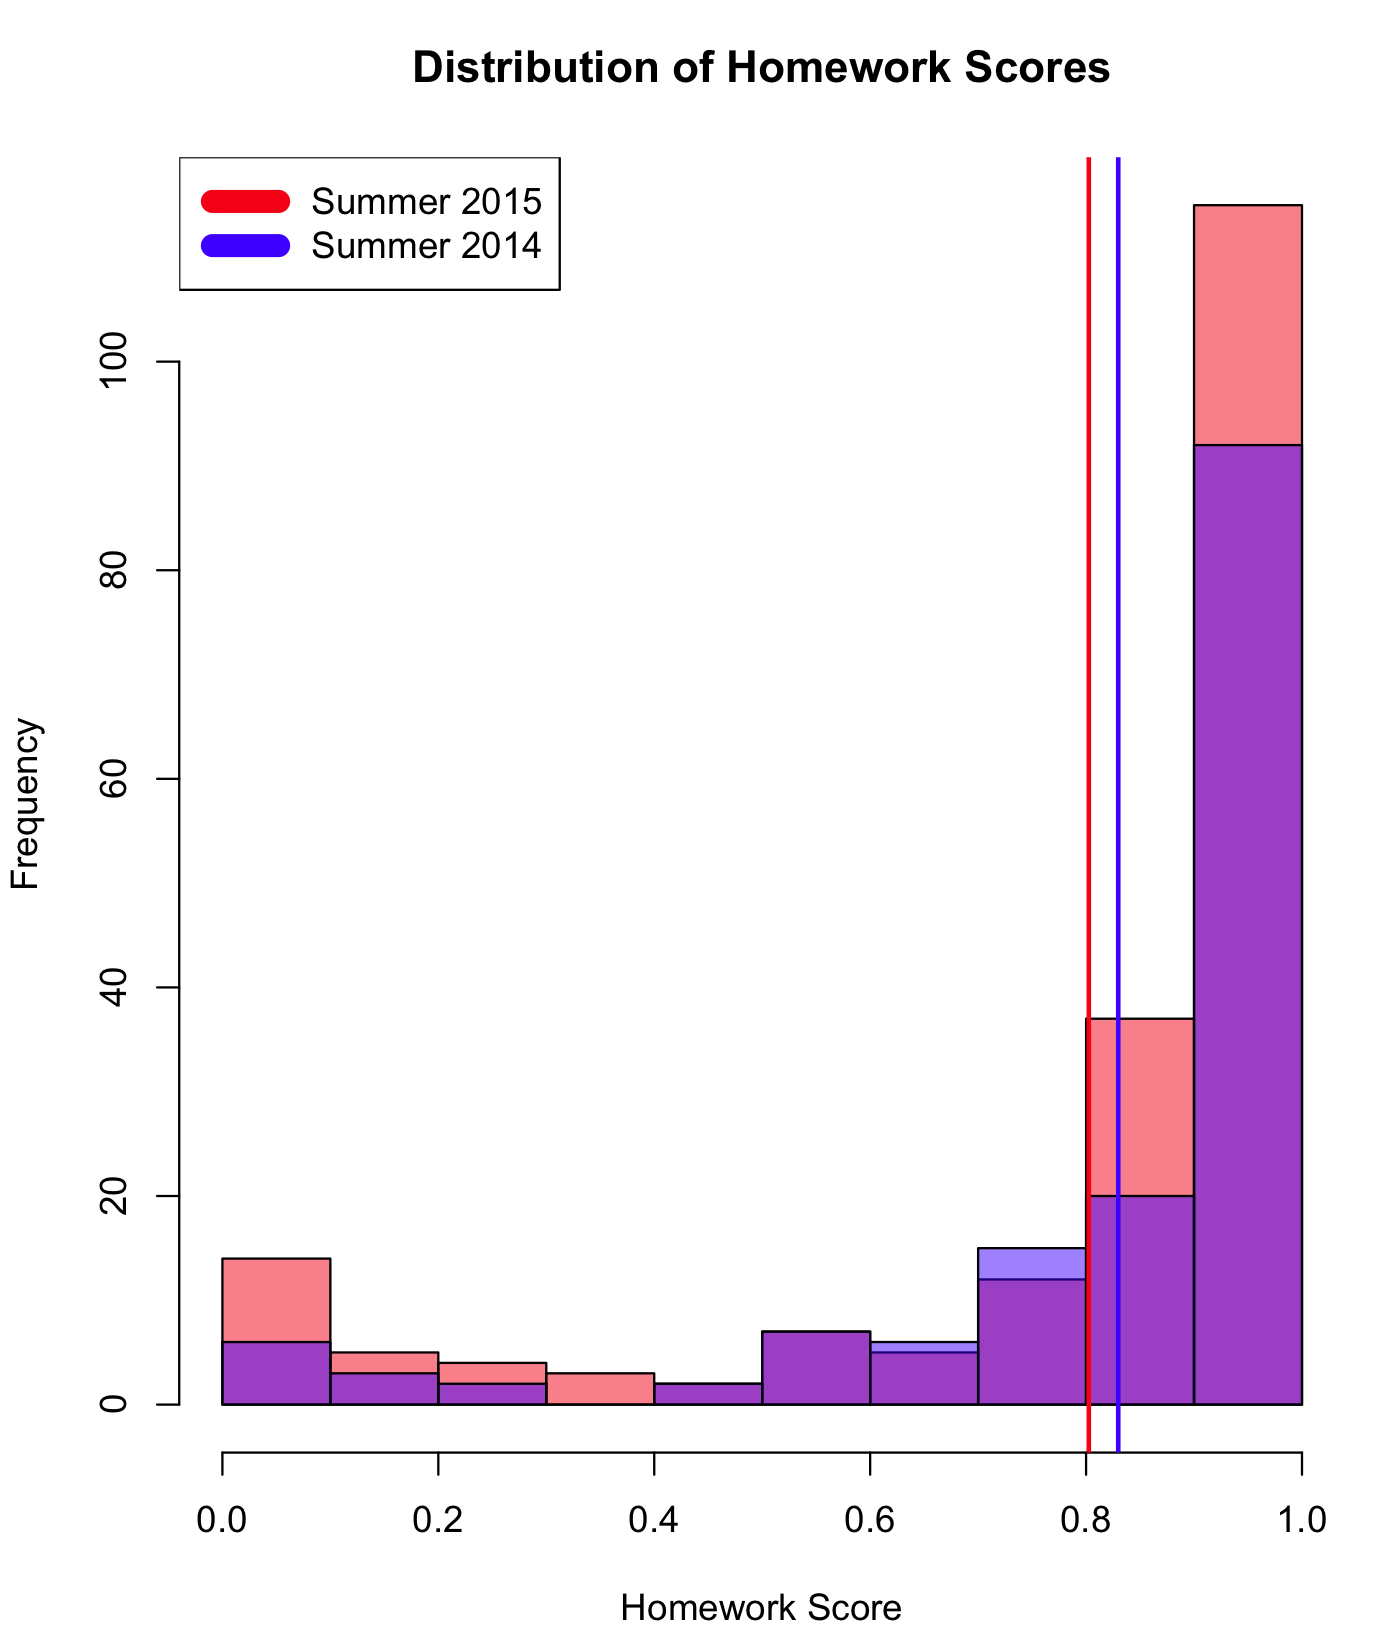
\includegraphics[width=2in]{img/chapter4/hw_su15_vs_su14}
\end{figure}
\end{column}
\begin{column}{2in}
\begin{scriptsize}
\begin{table}
  \begin{tabular}{|l|l|}
    \hline
    \textbf{Statistic} & \textbf{Value} \\
	\hline
	$\mu$ - 2015 & 0.803 \\
	\hline
	$\mu$ - 2014 & 0.830 \\
	\hline
	$\sigma$ - 2015 & 0.288 \\
	\hline
	$\sigma$ - 2014 & 0.242 \\
	\hline
	Shapiro-Wilk - 2015 & p $<$ 2.2e-16 \\
	\hline
	Shapiro-Wilk - 2014 & p $<$ 2.2e-16 \\
	\hline
	Wilcoxon Signed-Rank & p = 0.710 \\
	\hline
	Cohen's D & 0.101 \\
	\hline
  \end{tabular}
\end{table}
\end{scriptsize}
\end{column}
\end{columns}
\end{frame}

\begin{frame}{Fall 2014 vs. Summer 2015}
\begin{columns}
\begin{column}{2in}
\begin{figure}
	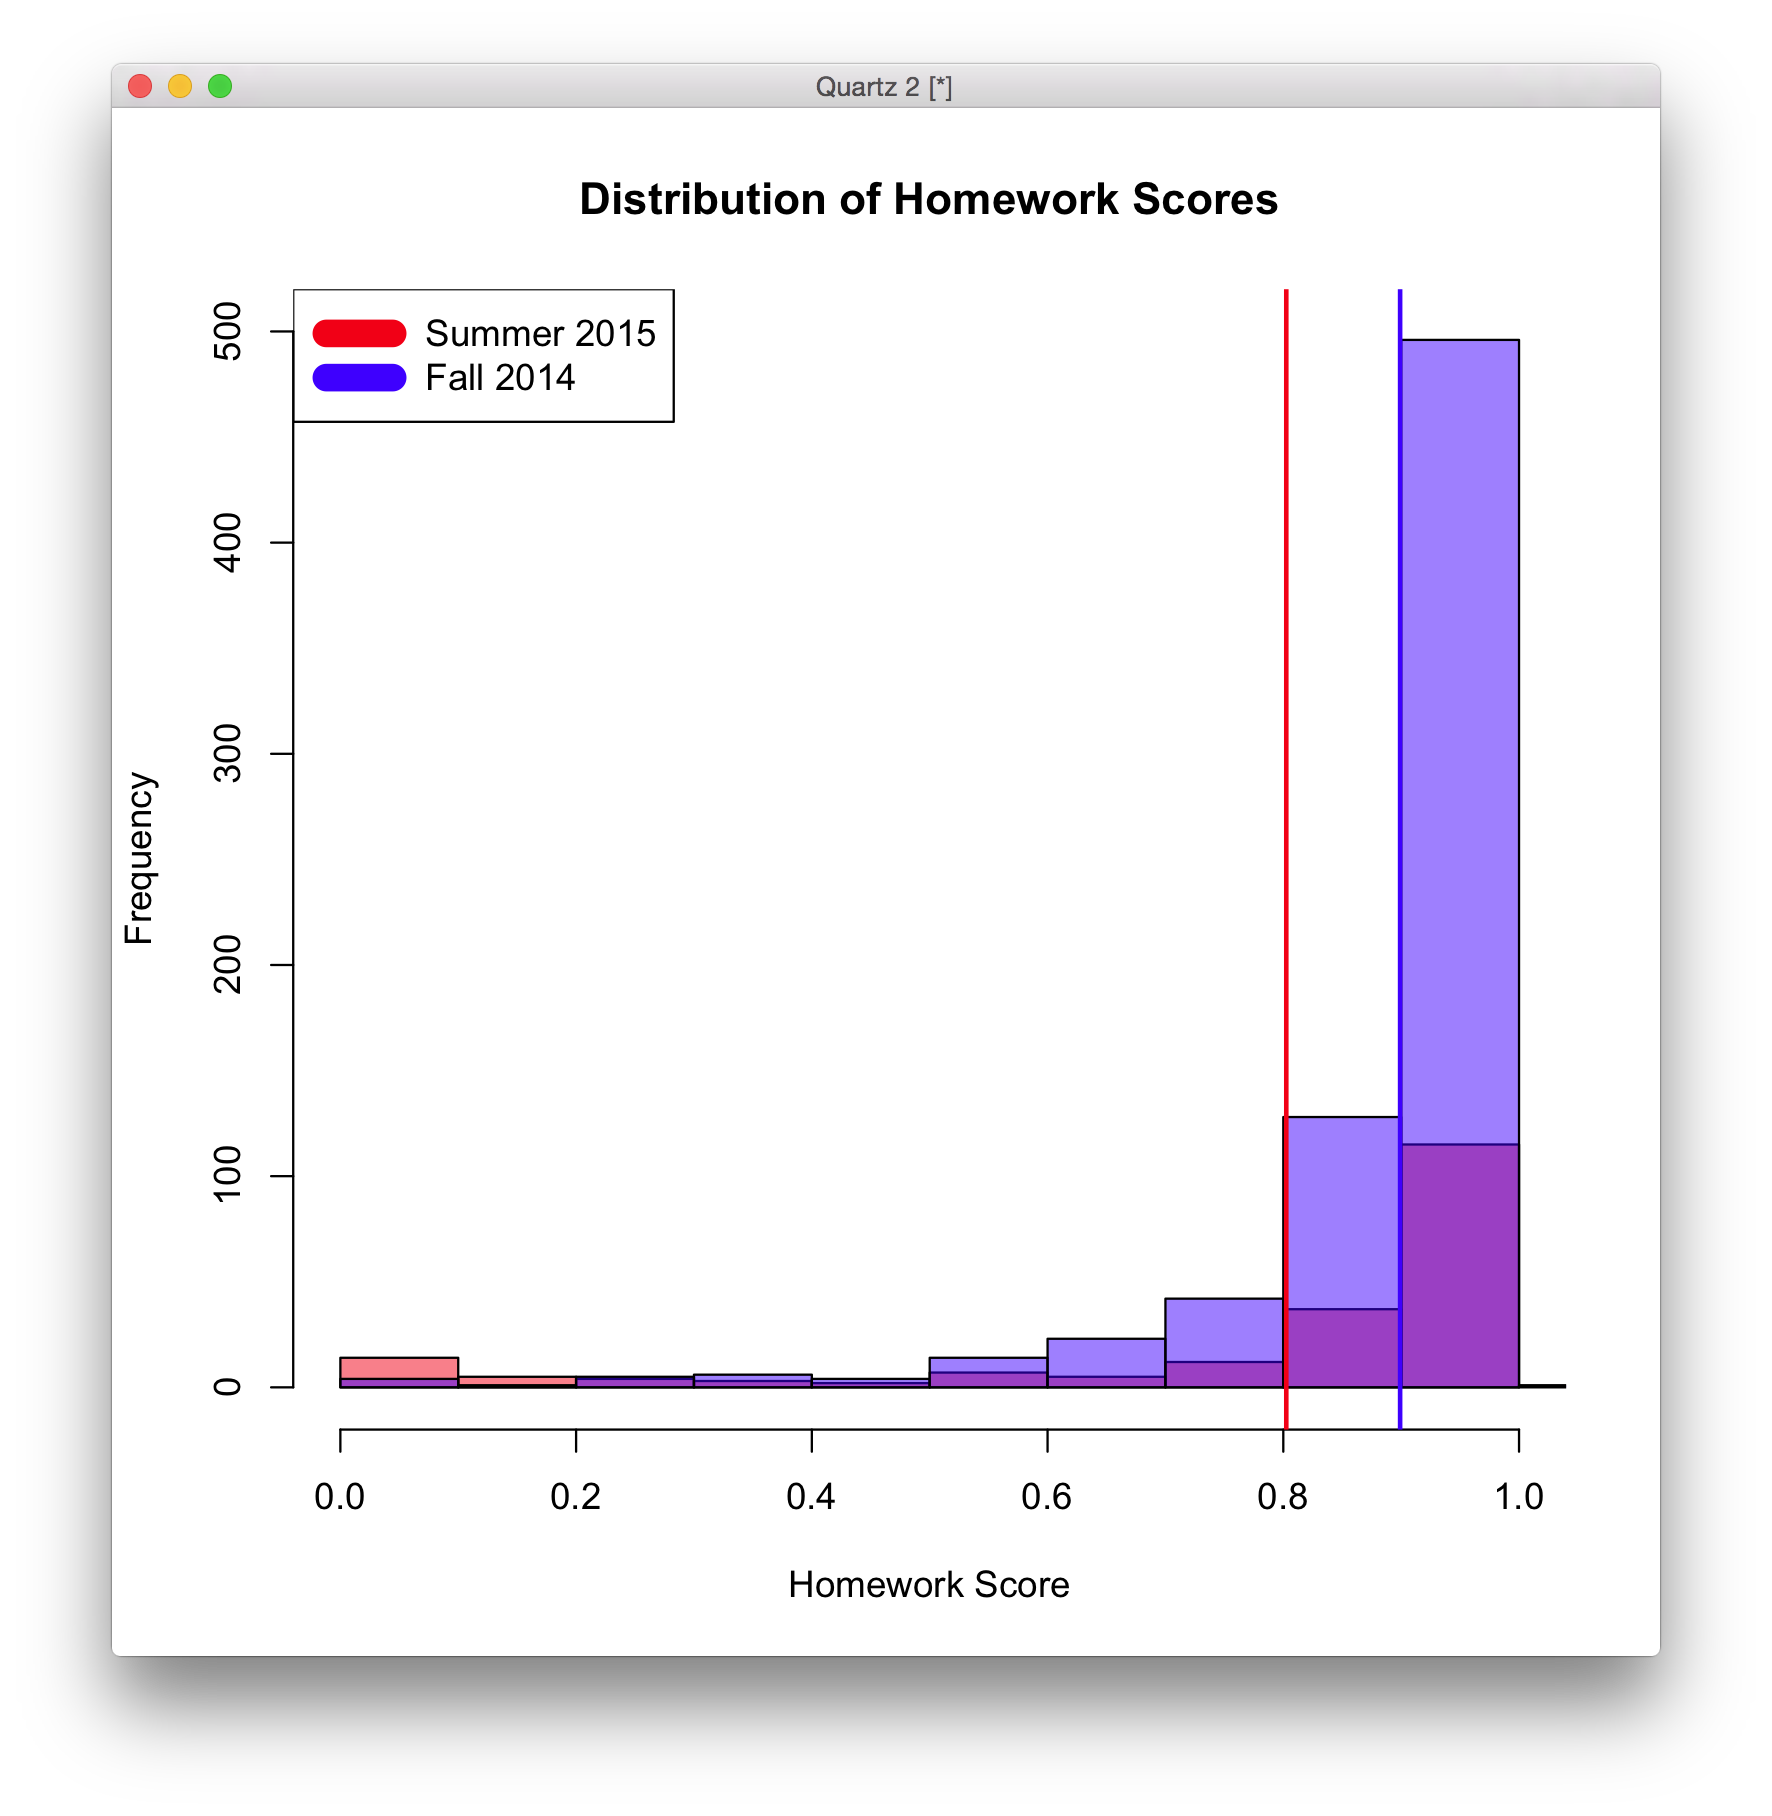
\includegraphics[width=2in]{img/chapter4/hw_su15_vs_f14}
\end{figure}
\end{column}
\begin{column}{2in}
\begin{scriptsize}
\begin{table}
  \begin{tabular}{|l|l|}
    \hline
    \textbf{Statistic} & \textbf{Value} \\
	\hline
	$\mu$ - 2015 & 0.803 \\
	\hline
	$\mu$ - 2014 & 0.899 \\
	\hline
	$\sigma$ - 2015 & 0.288 \\
	\hline
	$\sigma$ - 2014 & 0.144 \\
	\hline
	Shapiro-Wilk - 2015 & p $<$ 2.2e-16 \\
	\hline
	Shapiro-Wilk - 2014 & p $<$ 2.2e-16 \\
	\hline
	Wilcoxon Signed-Rank & p = 0.012 \\
	\hline
	Cohen's D & 0.5212 \\
	\hline
  \end{tabular}
\end{table}
\end{scriptsize}
\end{column}
\end{columns}
\end{frame}

\begin{frame}{Fall 2014 (Distance Learning) vs. Summer 2015}
\begin{columns}
\begin{column}{2in}
\begin{figure}
	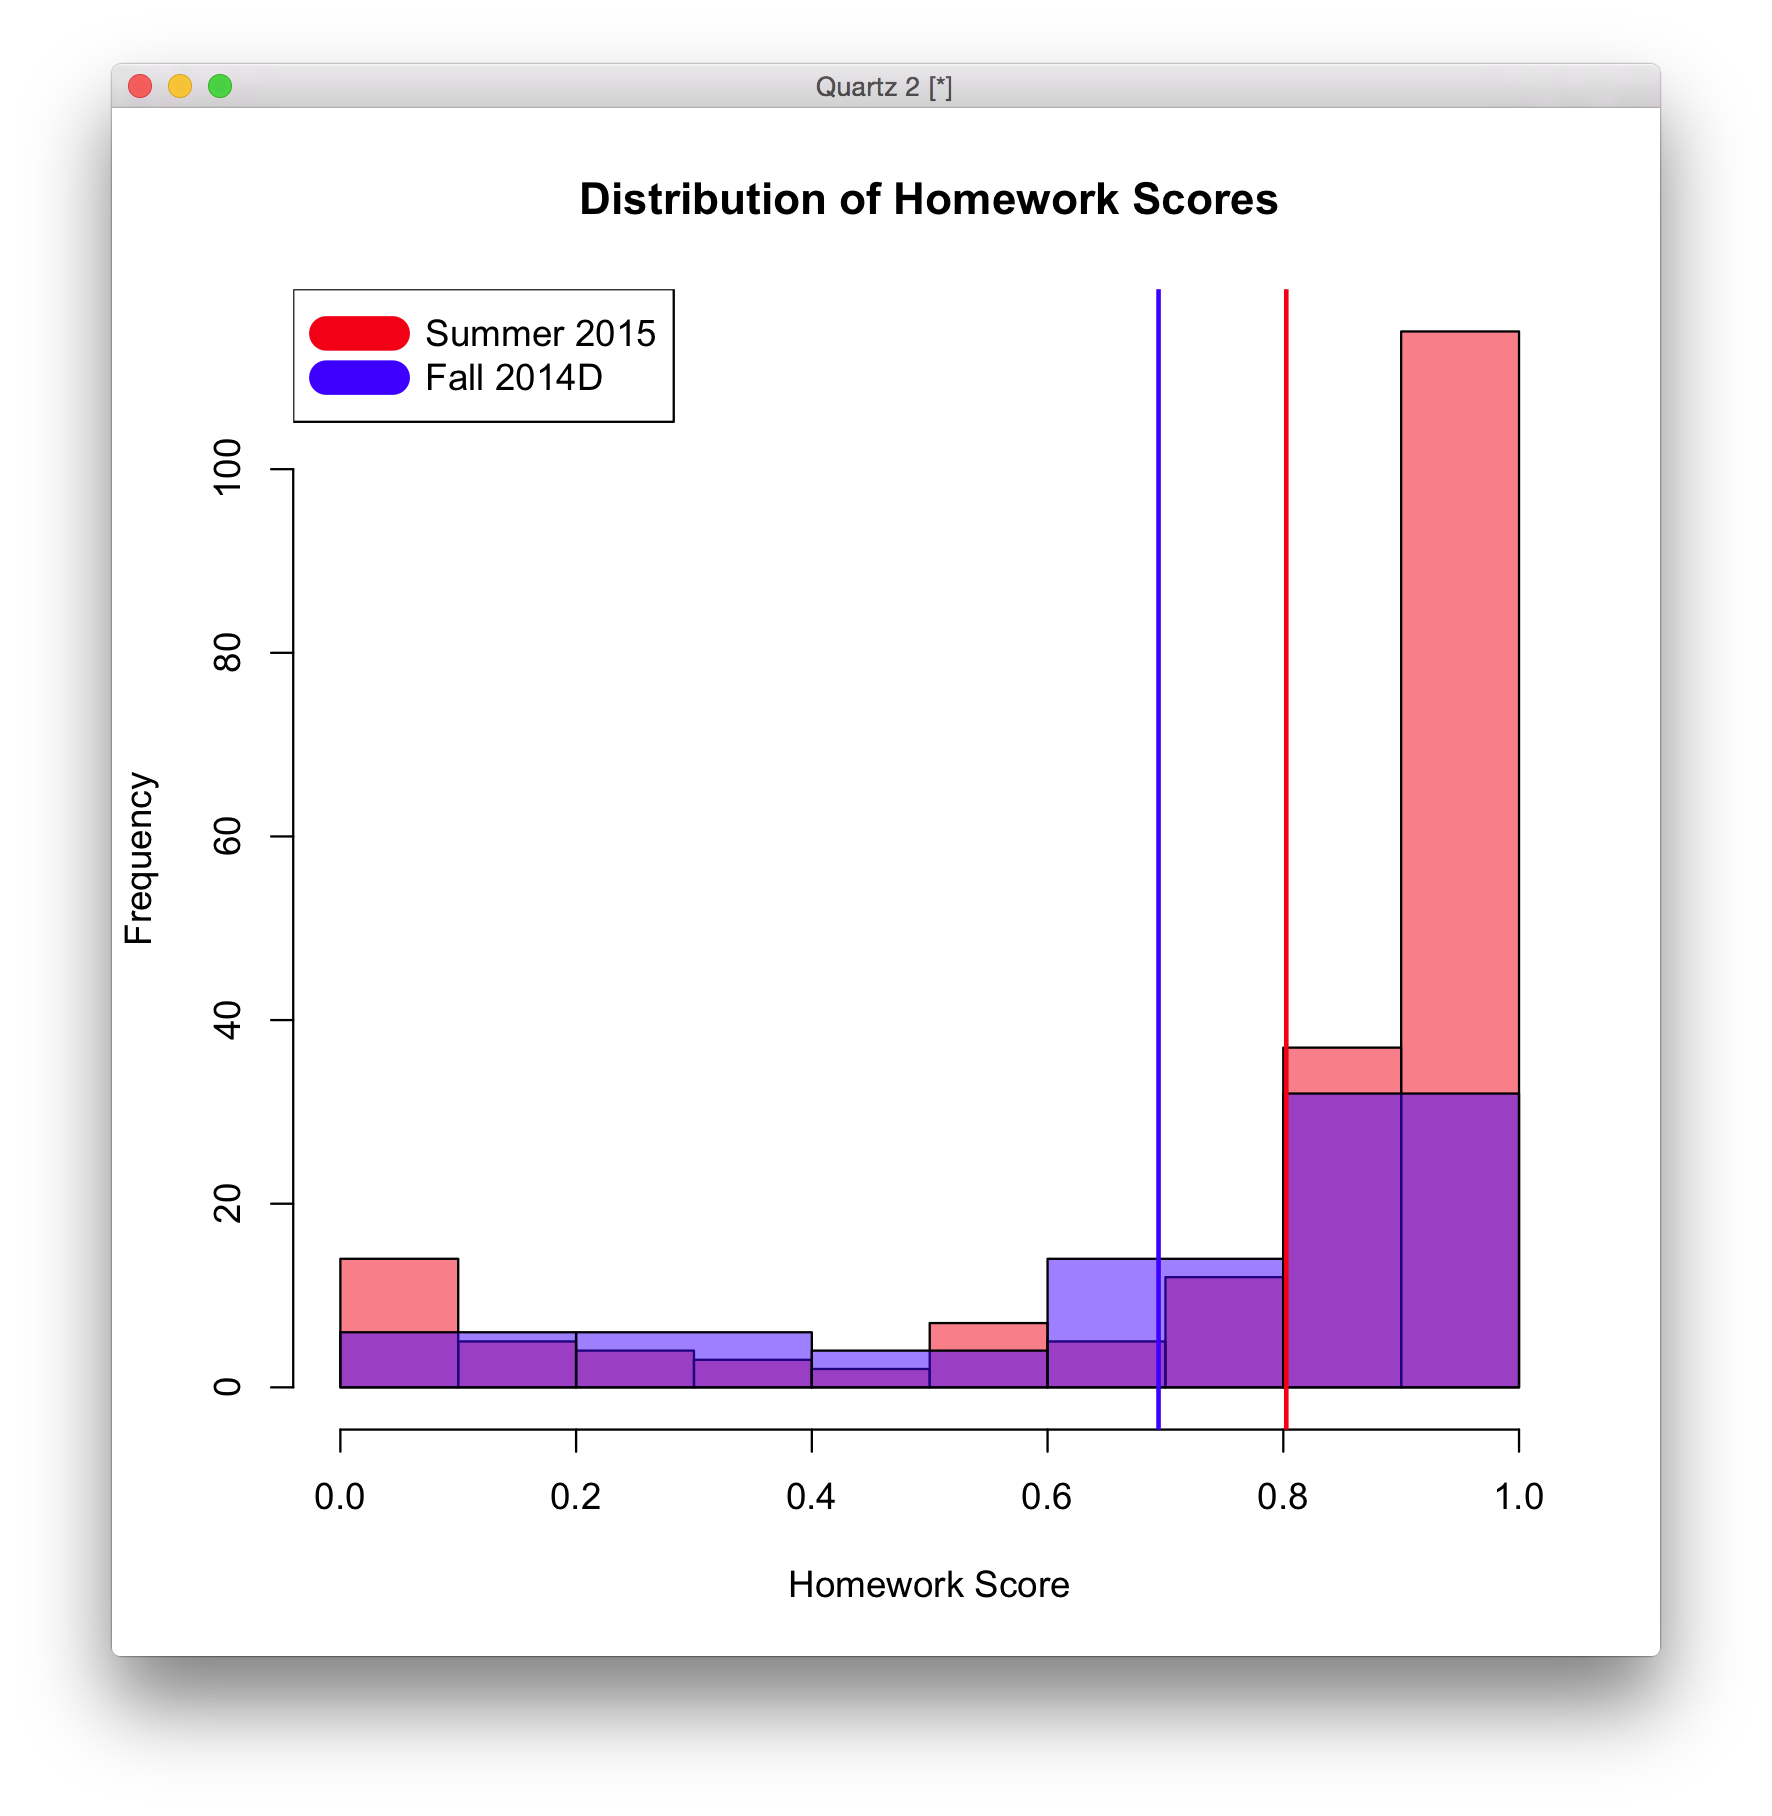
\includegraphics[width=2in]{img/chapter4/hw_su15_vs_f14d}
\end{figure}
\end{column}
\begin{column}{2in}
\begin{scriptsize}
\begin{table}
  \begin{tabular}{|l|l|}
    \hline
    \textbf{Statistic} & \textbf{Value} \\
	\hline
	$\mu$ - 2015 & 0.803 \\
	\hline
	$\mu$ - 2014 & 0.694 \\
	\hline
	$\sigma$ - 2015 & 0.288 \\
	\hline
	$\sigma$ - 2014 & 0.296 \\
	\hline
	Shapiro-Wilk - 2015 & p $<$ 2.2e-16 \\
	\hline
	Shapiro-Wilk - 2014 & p = 9.146e-07 \\
	\hline
	Wilcoxon Signed-Rank & p = 3.726e-05 \\
	\hline
	Cohen's D & 0.374 \\
	\hline
  \end{tabular}
\end{table}
\end{scriptsize}
\end{column}
\end{columns}
\end{frame}

\begin{frame}{Spring 2015 vs. Summer 2015}
\begin{columns}
\begin{column}{2in}
\begin{figure}
	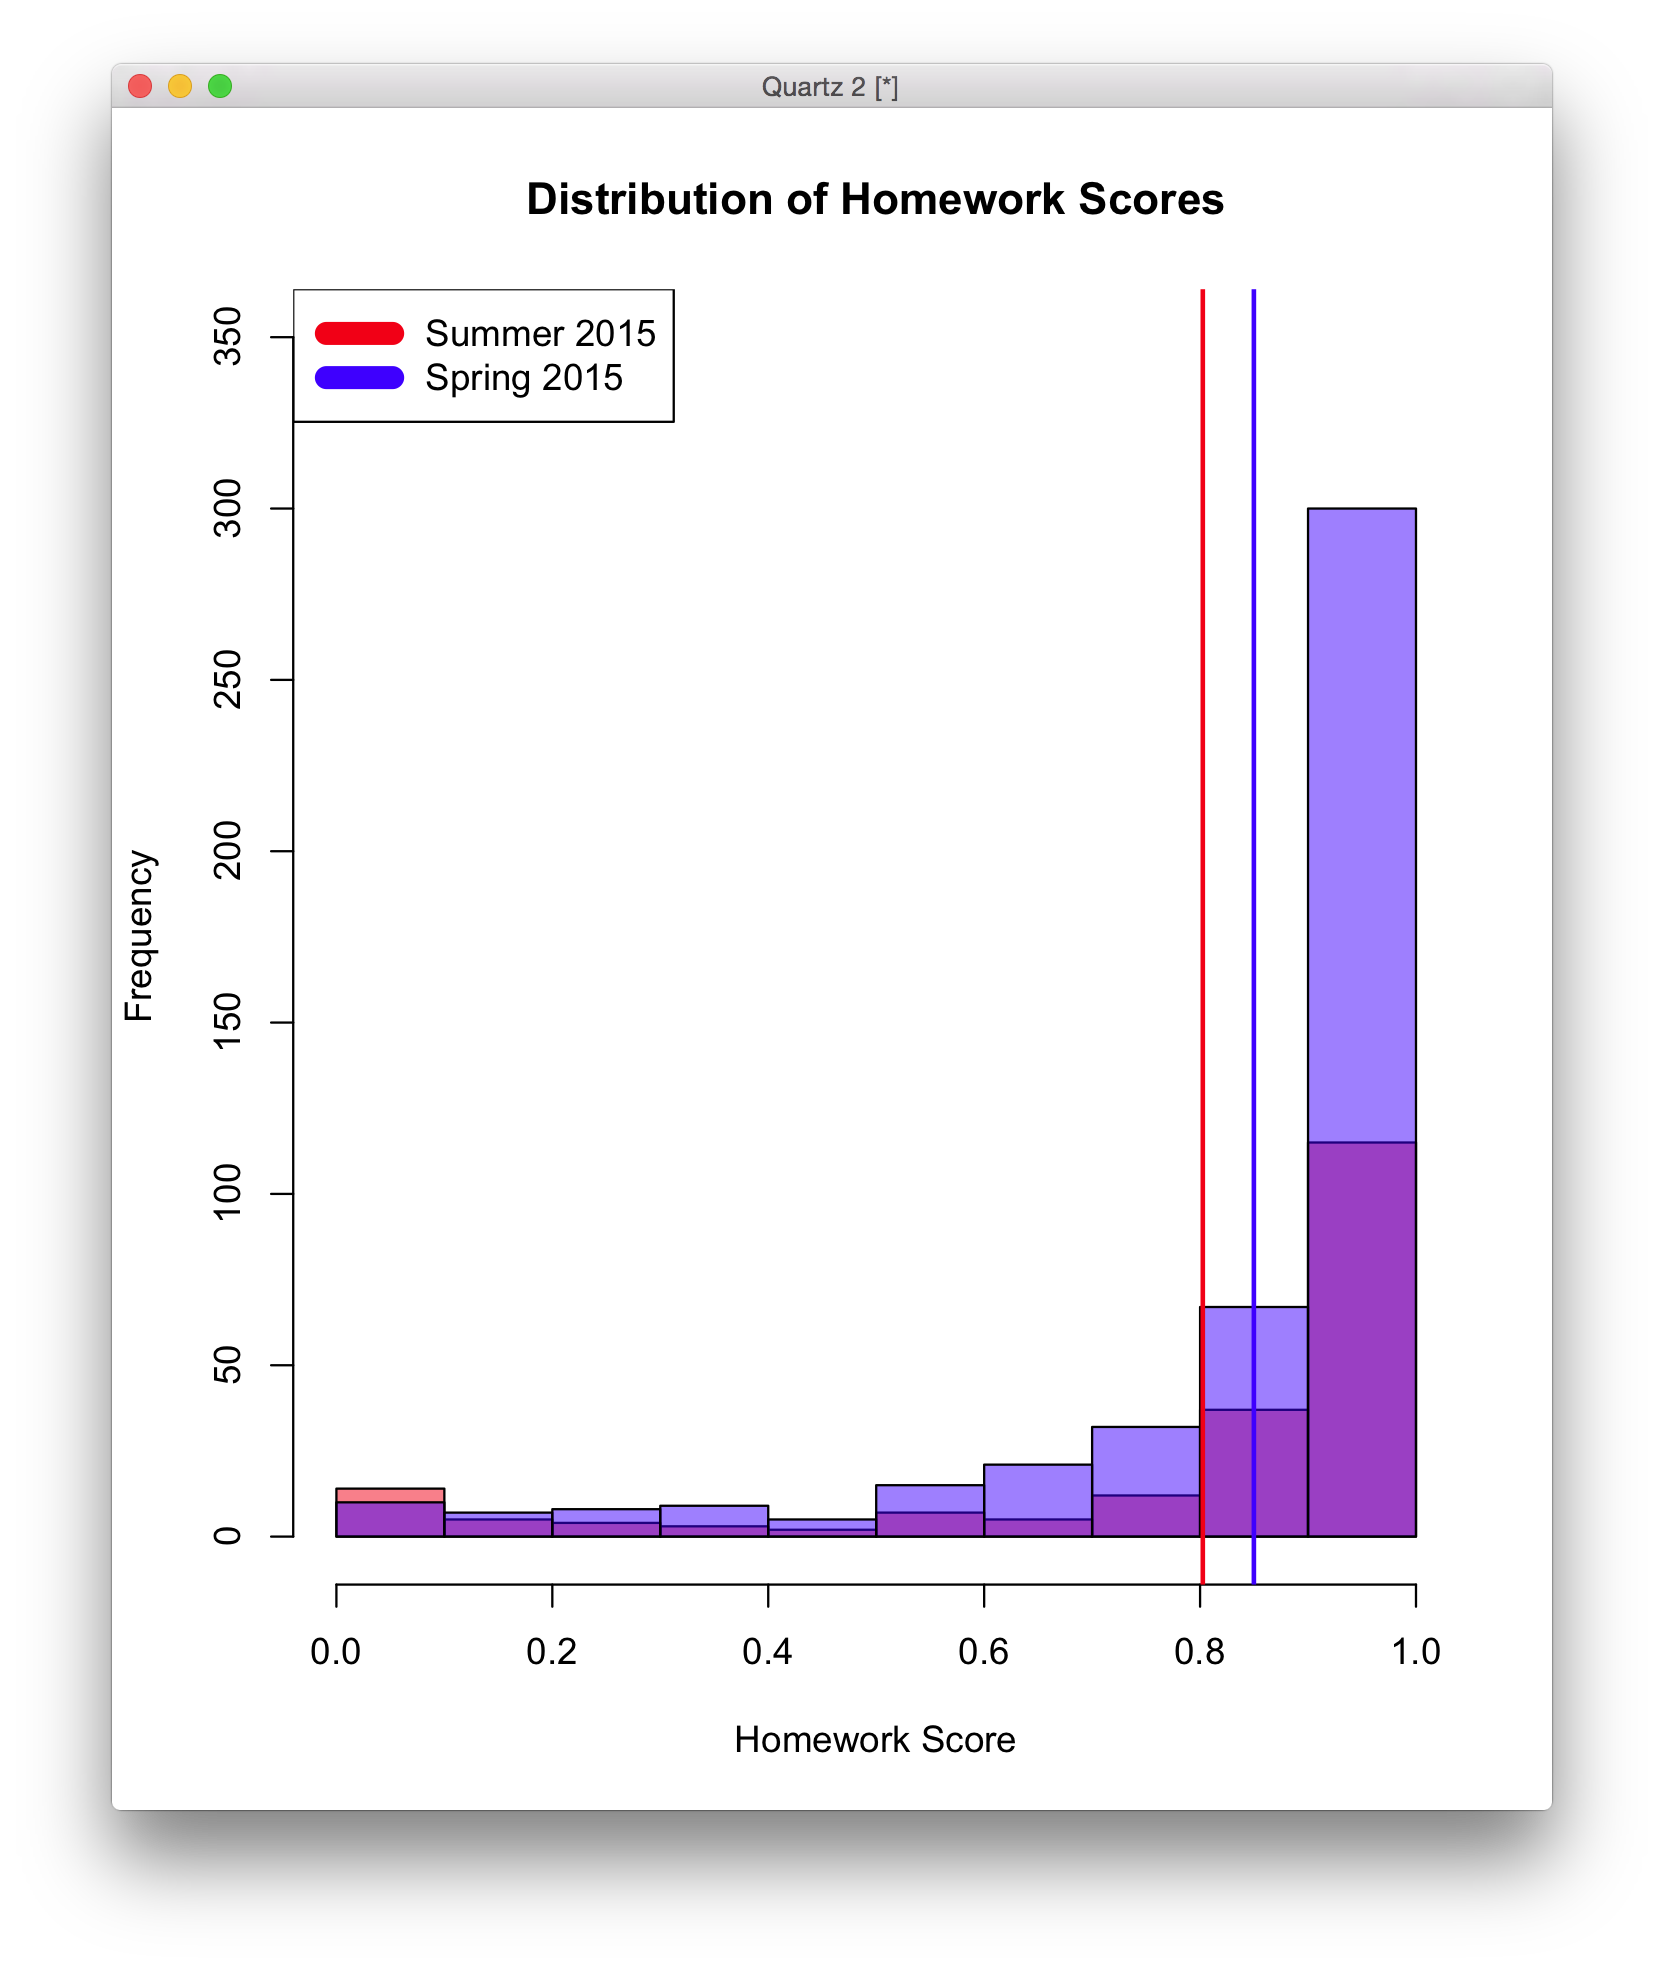
\includegraphics[width=2in]{img/chapter4/hw_su15_vs_sp15}
\end{figure}
\end{column}
\begin{column}{2in}
\begin{scriptsize}
\begin{table}
  \begin{tabular}{|l|l|}
    \hline
    \textbf{Statistic} & \textbf{Value} \\
	\hline
	$\mu$ - Su 2015 & 0.803 \\
	\hline
	$\mu$ - Sp 2015 & 0.850 \\
	\hline
	$\sigma$ - Su 2015 & 0.288 \\
	\hline
	$\sigma$ - Sp 2015 & 0.220 \\
	\hline
	Shapiro-Wilk - Su 2015 & p $<$ 2.2e-16 \\
	\hline
	Shapiro-Wilk - Sp 2015 & p $<$ 2.2e-16 \\
	\hline
	Wilcoxon Signed-Rank & p = 0.4551 \\
	\hline
	Cohen's D & 0.195 \\
	\hline
  \end{tabular}
\end{table}
\end{scriptsize}
\end{column}
\end{columns}
\end{frame}

\begin{frame}{Spring 2015 (Distance Learning) vs. Summer 2015}
\begin{columns}
\begin{column}{2in}
\begin{figure}
	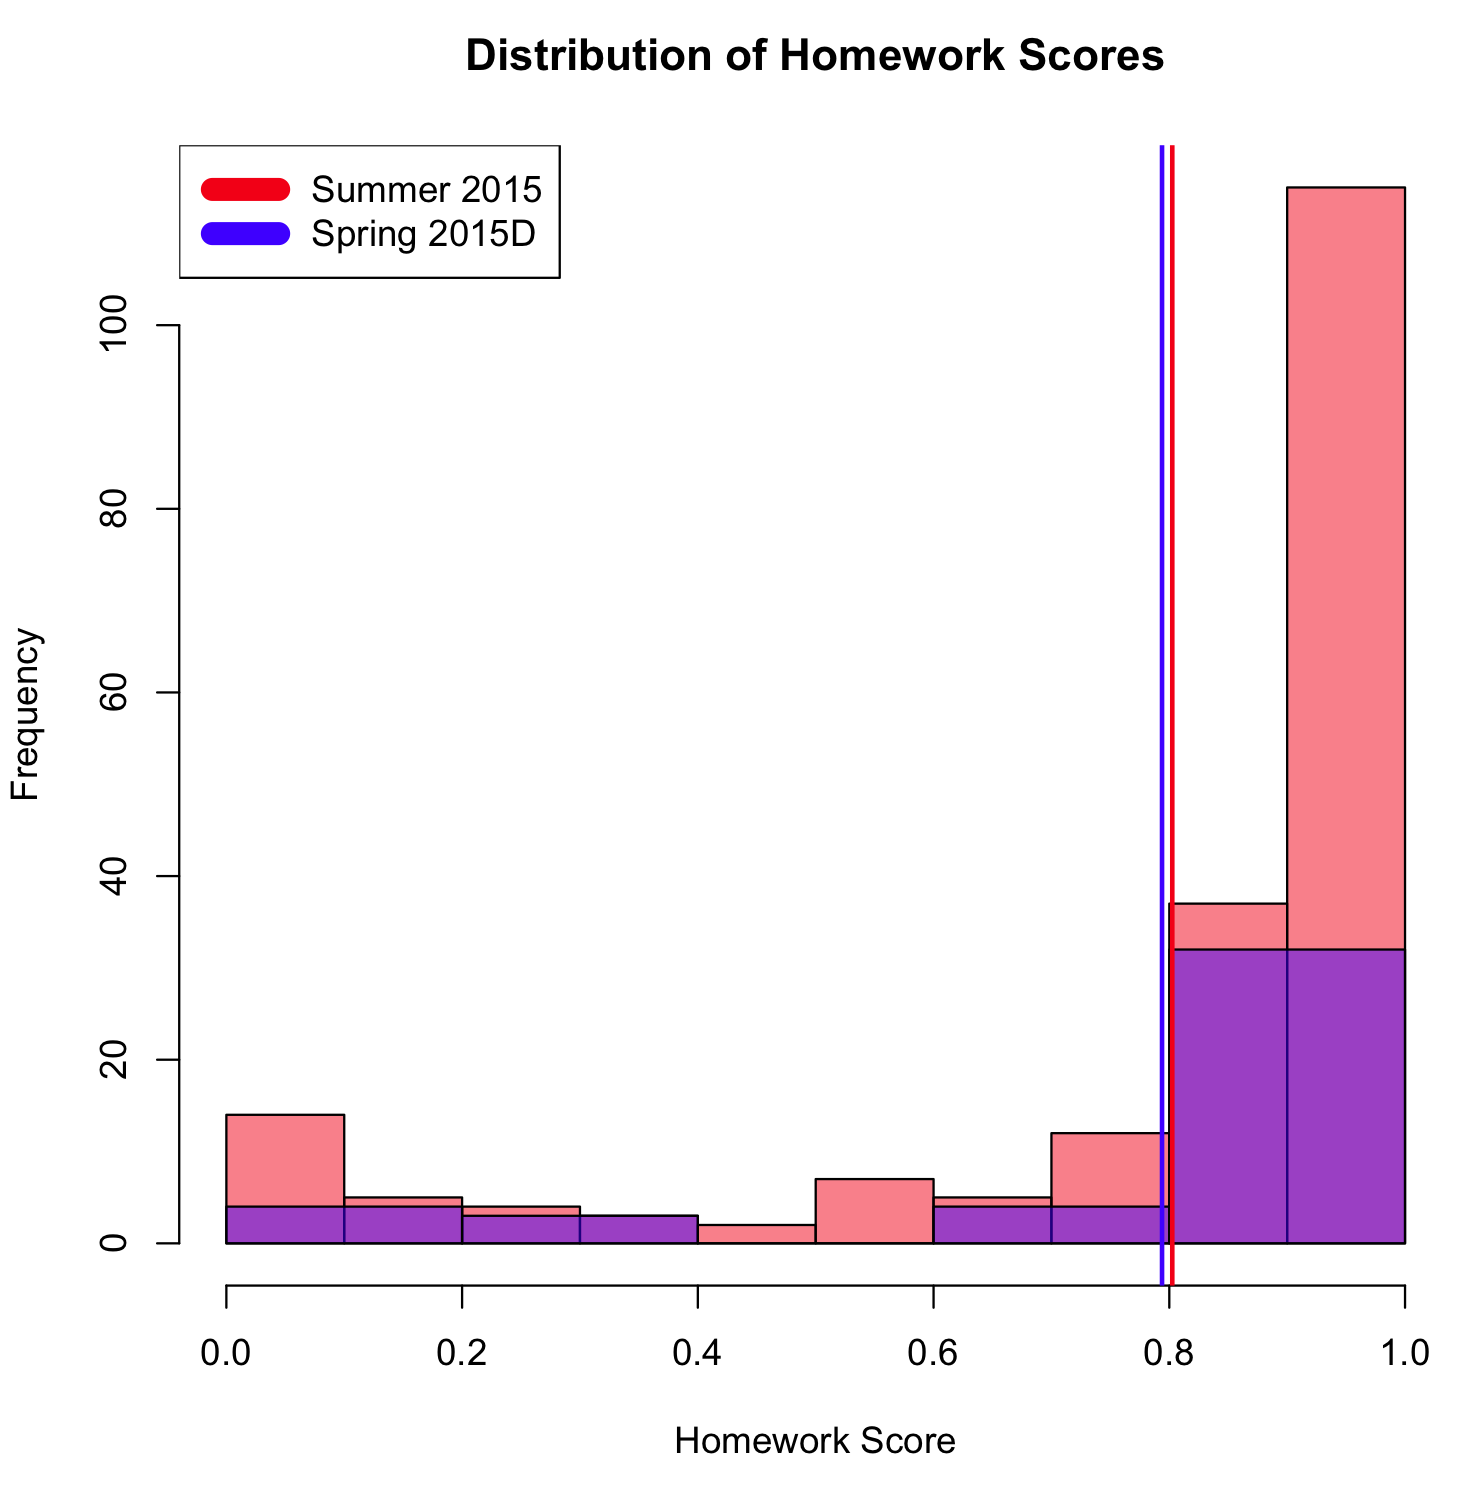
\includegraphics[width=2in]{img/chapter4/hw_su15_vs_sp15d}
\end{figure}
\end{column}
\begin{column}{2in}
\begin{scriptsize}
\begin{table}
  \begin{tabular}{|l|l|}
    \hline
    \textbf{Statistic} & \textbf{Value} \\
	\hline
	$\mu$ - Su 2015 & 0.803 \\
	\hline
	$\mu$ - Sp 2015 & 0.794 \\
	\hline
	$\sigma$ - Su 2015 & 0.288 \\
	\hline
	$\sigma$ - Sp 2015 & 0.294 \\
	\hline
	Shapiro-Wilk - Su 2015 & p $<$ 2.2e-16 \\
	\hline
	Shapiro-Wilk - Sp 2015 & p = 2.166e-08 \\
	\hline
	Wilcoxon Signed-Rank & p = 0.7237 \\
	\hline
	Cohen's D & 0.030 \\
	\hline
  \end{tabular}
\end{table}
\end{scriptsize}
\end{column}
\end{columns}
\end{frame}

\begin{frame}{Trends with Homework Scores}
  \begin{itemize}
    \item The CITA program seems to improve homework scores in online classes.
    \item Even with the score boost, online classes with CITA still behind the on-campus classes.
  \end{itemize}
\end{frame}

%%%%%%%%%%%%
% Recitation Quizzes %
%%%%%%%%%%%%
\subsection*{Recitation Quizzes}

\begin{frame}{Overview of Recitation Quizzes}
  \begin{itemize}
    \item Recitation quizzes are five question quizzes given to students during or after recitation.
    \item They are used for a wide variety of purposes (warm-ups, teaching material, recording attendance, etc.).
    \item They are administered online through CHIP in the form of a timed multiple choice test for the online classes.
    \item The online recitation quizzes are an excellent benchmark in this study because they did not change between summer 2014 and summer 2015.
  \end{itemize}
\end{frame}

\begin{frame}{Summer 2014 vs. Summer 2015}
\begin{columns}
\begin{column}{2in}
\begin{figure}
	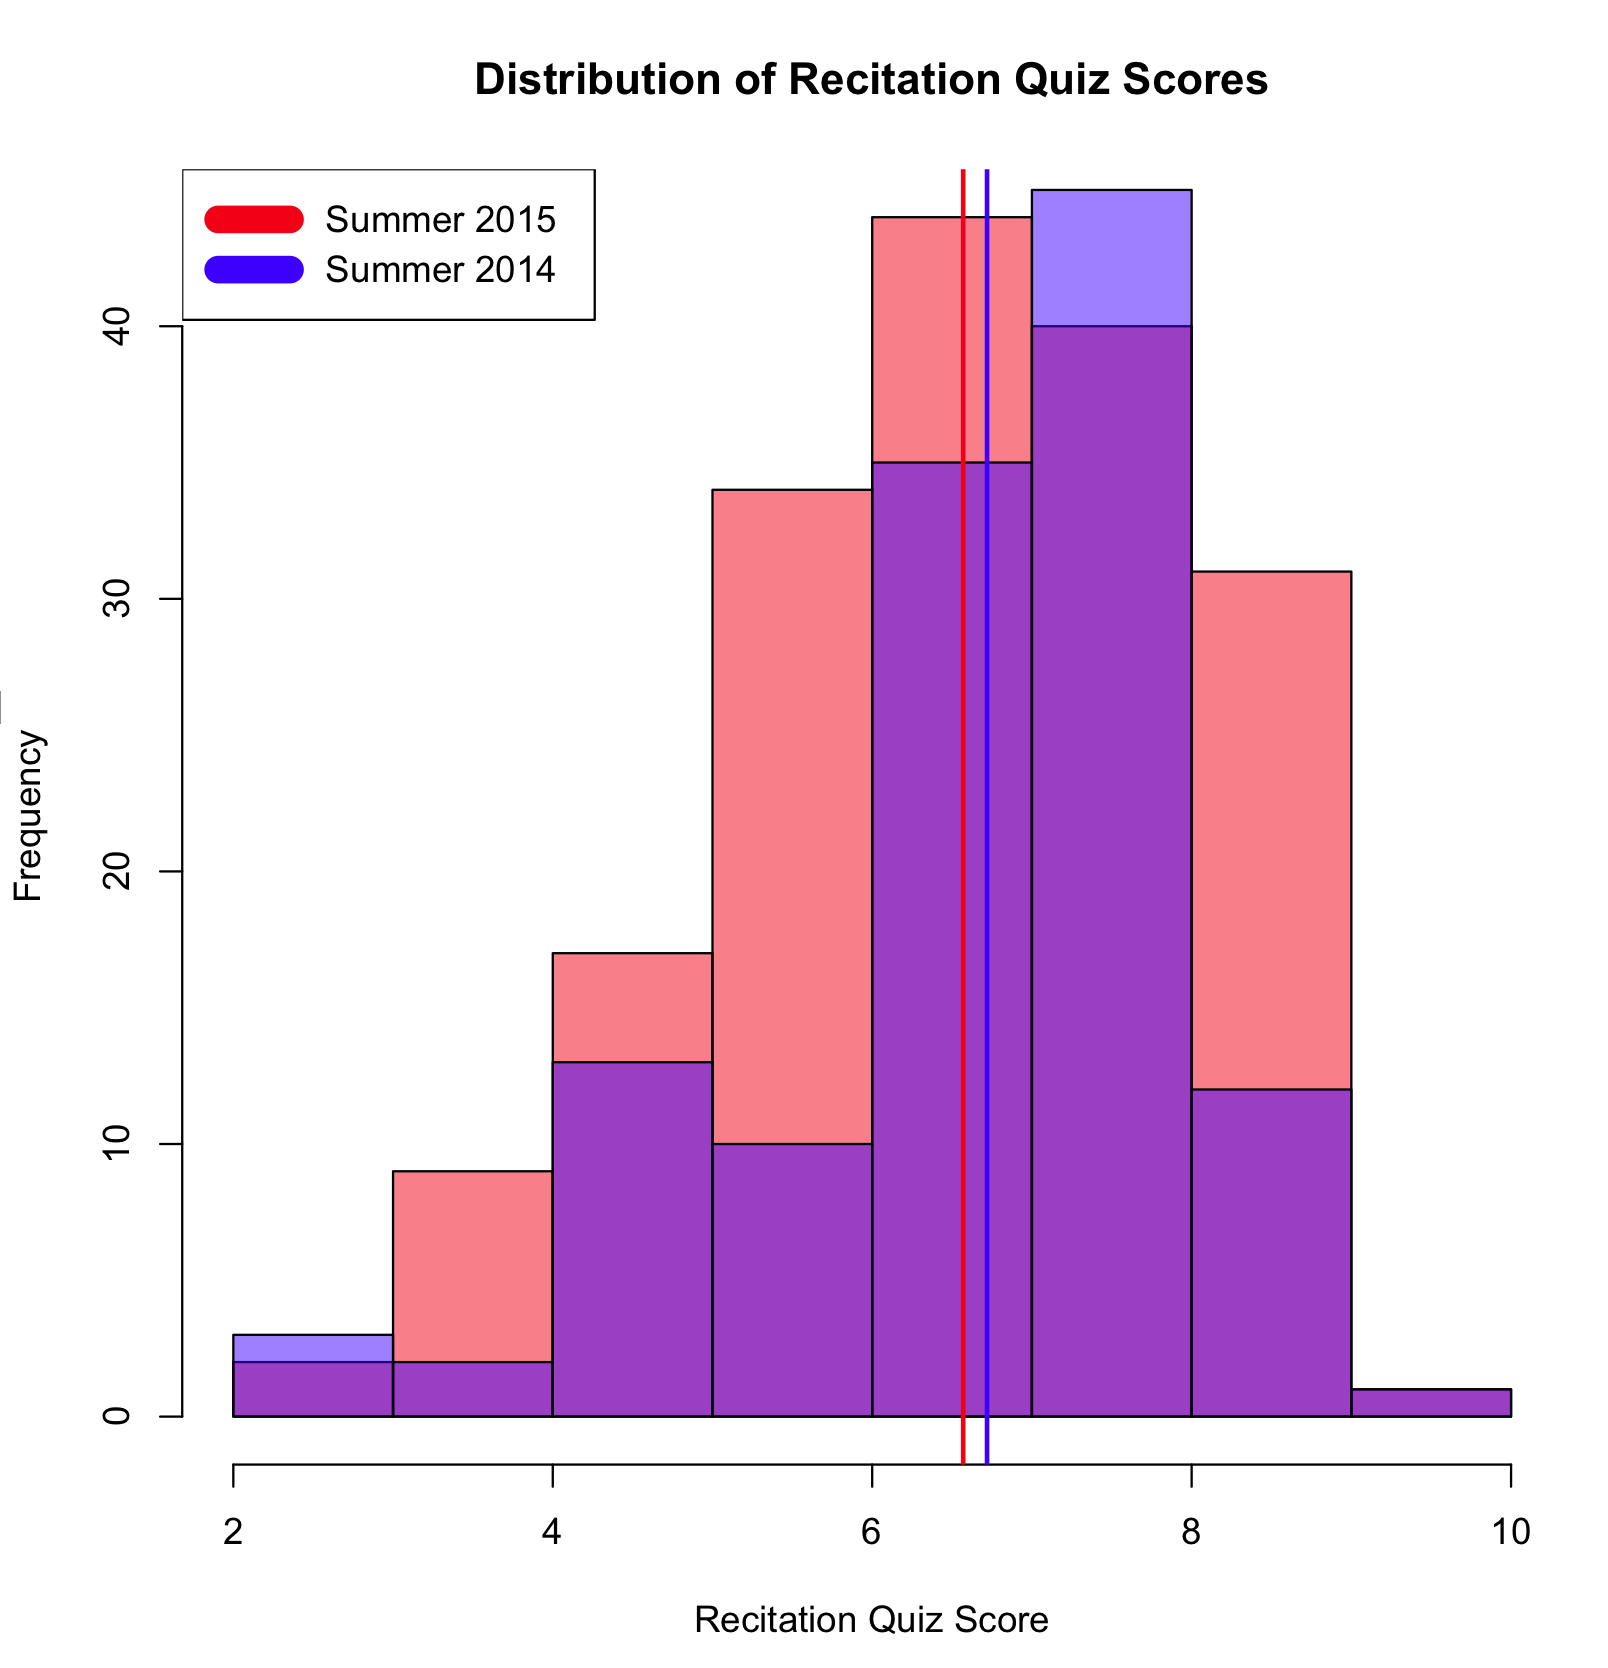
\includegraphics[width=2in]{img/chapter4/rq_su15_vs_su14}
\end{figure}
\end{column}
\begin{column}{2in}
\begin{scriptsize}
\begin{table}
  \begin{tabular}{|l|l|}
    \hline
    \textbf{Statistic} & \textbf{Value} \\
	\hline
	$\mu$ - 2015 & 6.570 \\
	\hline
	$\mu$ - 2014 & 6.719 \\
	\hline
	$\sigma$ - 2015 & 1.485 \\
	\hline
	$\sigma$ - 2014 & 1.378 \\
	\hline
	Shapiro-Wilk - 2015 & p = 0.0006211 \\
	\hline
	Shapiro-Wilk - 2014 & p = 1.508e-05 \\
	\hline
	Wilcoxon Signed-Rank & p = 0.3848 \\
	\hline
	Cohen's D & 0.103 \\
	\hline
  \end{tabular}
\end{table}
\end{scriptsize}
\end{column}
\end{columns}
\end{frame}

\begin{frame}{Fall 2014 (Distance Learning) vs. Summer 2015}
\begin{columns}
\begin{column}{2in}
\begin{figure}
	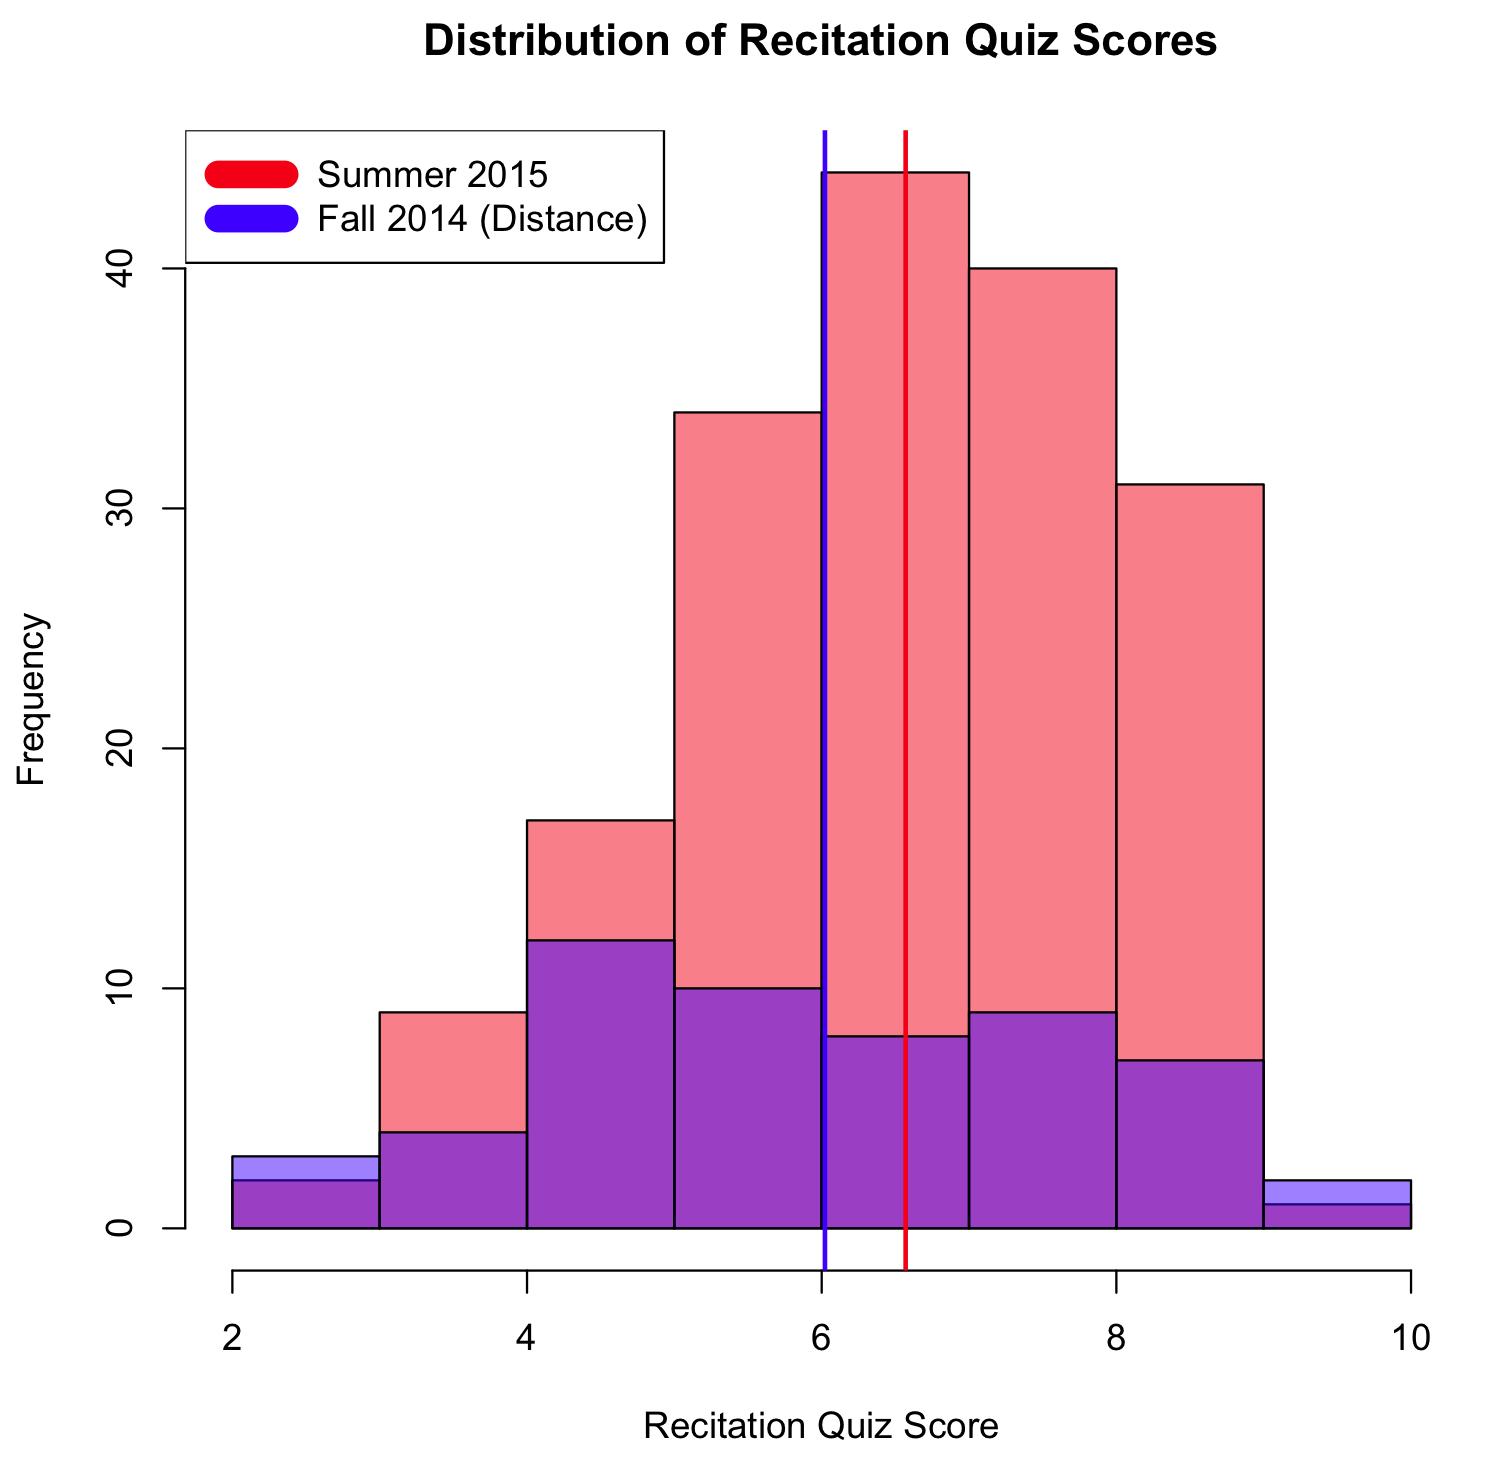
\includegraphics[width=2in]{img/chapter4/rq_su15_vs_f14d}
\end{figure}
\end{column}
\begin{column}{2in}
\begin{scriptsize}
\begin{table}
  \begin{tabular}{|l|l|}
    \hline
    \textbf{Statistic} & \textbf{Value} \\
	\hline
	$\mu$ - 2015 & 6.570 \\
	\hline
	$\mu$ - 2014 & 6.022 \\
	\hline
	$\sigma$ - 2015 & 1.485 \\
	\hline
	$\sigma$ - 2014 & 1.786 \\
	\hline
	Shapiro-Wilk - 2015 & p = 0.0006211 \\
	\hline
	Shapiro-Wilk - 2014 & p = 0.6931 \\
	\hline
	Wilcoxon Signed-Rank & p = 0.02972 \\
	\hline
	Cohen's D & 0.351 \\
	\hline
  \end{tabular}
\end{table}
\end{scriptsize}
\end{column}
\end{columns}
\end{frame}

\begin{frame}{Spring 2015 (Distance Learning) vs. Summer 2015}
\begin{columns}
\begin{column}{2in}
\begin{figure}
	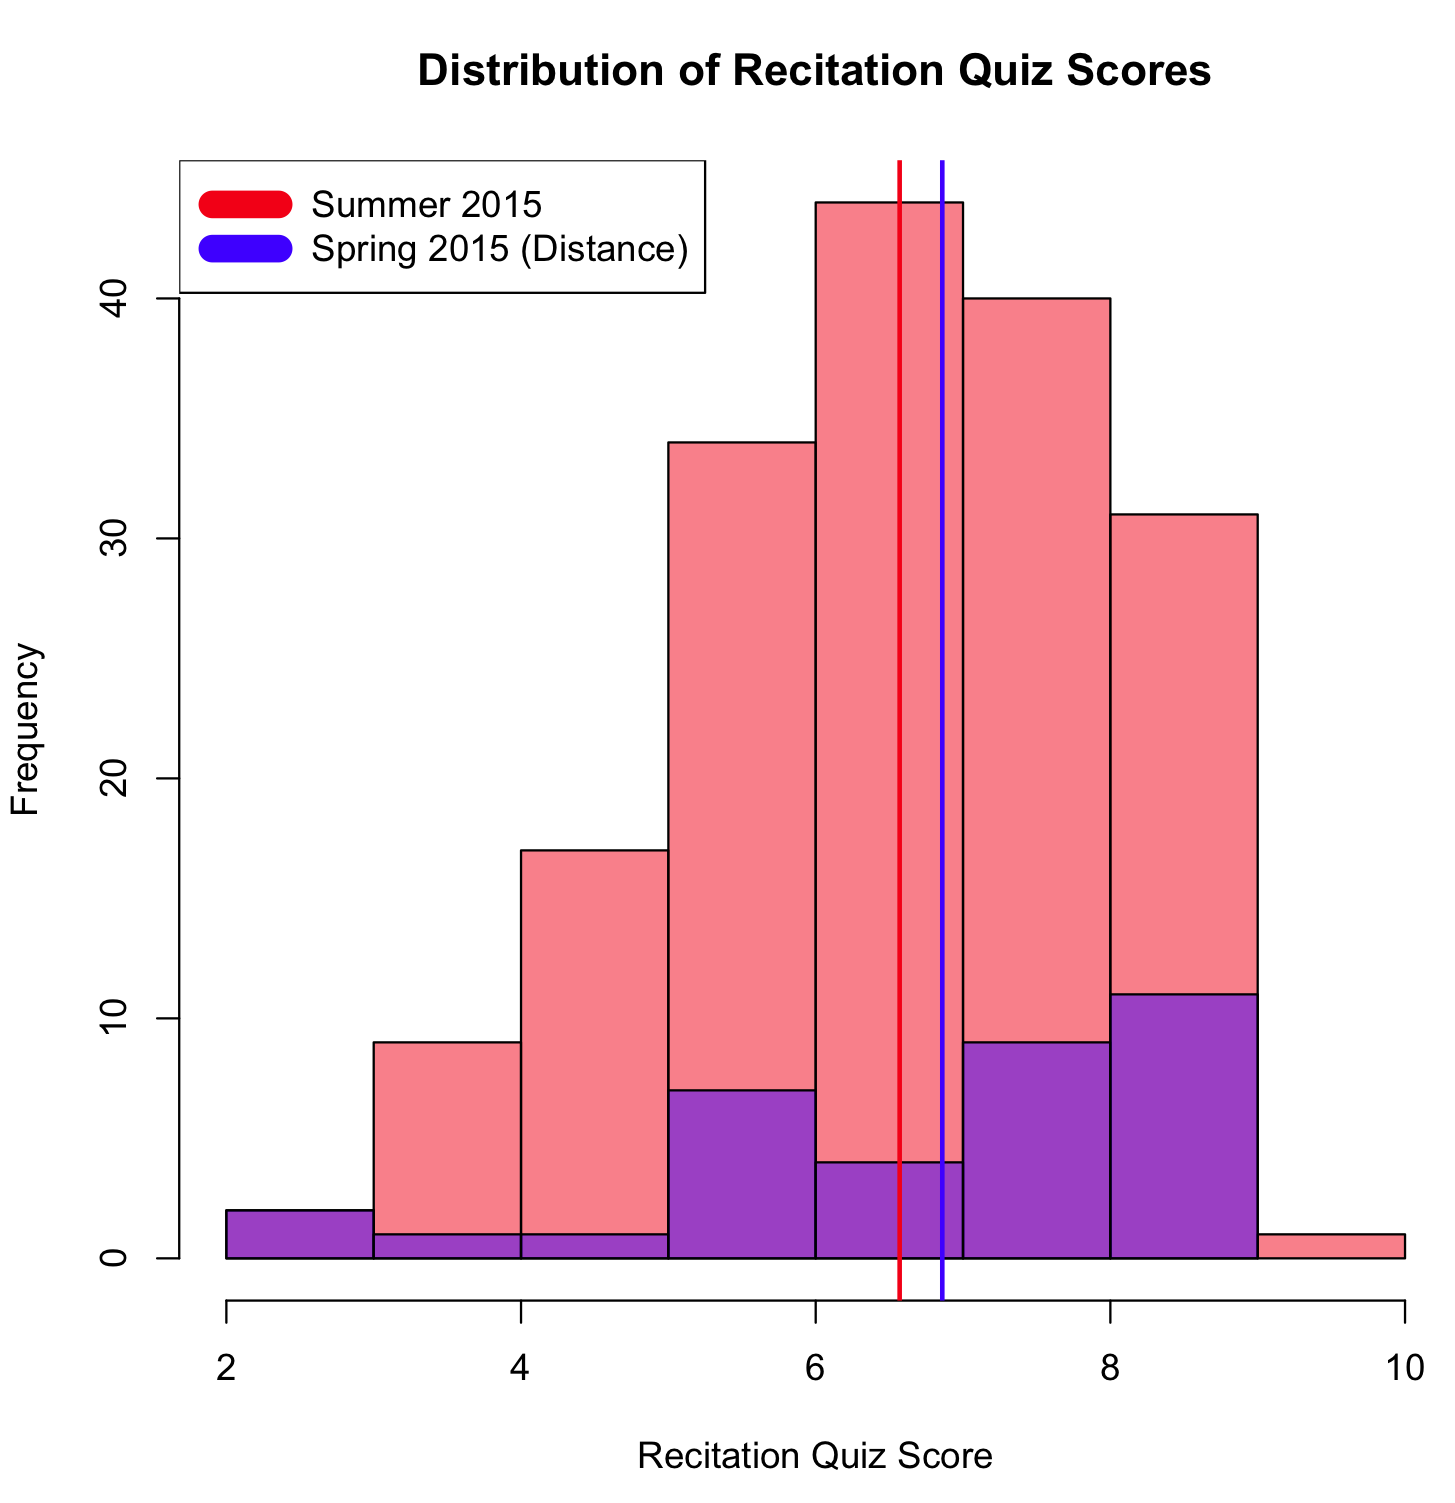
\includegraphics[width=2in]{img/chapter4/rq_su15_vs_sp15d}
\end{figure}
\end{column}
\begin{column}{2in}
\begin{scriptsize}
\begin{table}
  \begin{tabular}{|l|l|}
    \hline
    \textbf{Statistic} & \textbf{Value} \\
	\hline
	$\mu$ - Su 2015 & 6.570 \\
	\hline
	$\mu$ - Sp 2015 & 6.859 \\
	\hline
	$\sigma$ - Su 2015 & 1.485 \\
	\hline
	$\sigma$ - Sp 2015 & 1.643 \\
	\hline
	Shapiro-Wilk - Su 2015 & p = 0.0006211 \\
	\hline
	Shapiro-Wilk - Sp 2015 & p = 0.005266 \\
	\hline
	Wilcoxon Signed-Rank & p = 0.1716 \\
	\hline
	Cohen's D & 0.191 \\
	\hline
  \end{tabular}
\end{table}
\end{scriptsize}
\end{column}
\end{columns}
\end{frame}

\begin{frame}{Trends with Recitation Quiz Scores}
  \begin{itemize}
    \item Summer 2015 recitation quiz scores are comparable to those in summer 2014 and spring 2015.
    \item The mean summer 2015 recitation quiz score is significantly different from that of fall 2014 (with a small effect size).
    \item Recitation quiz scores either stayed the same or increased slightly.
  \end{itemize}
\end{frame}

%%%%%%%%%%%
% Lecture Quizzes %
%%%%%%%%%%%
\subsection*{Lecture Quizzes}

\begin{frame}{Overview of Lecture Quizzes}
  \begin{itemize}
    \item Lecture quizzes are short quizzes given to students to test their knowledge of the readings.
    \item They are often used with i>Clickers to supplement lectures.
    \item They are also be administered online through CHIP in the form of a timed multiple choice test.
    \item The online lecture quizzes are an excellent benchmark in this study because they did not change between summer 2014 and summer 2015.
  \end{itemize}
\end{frame}

\begin{frame}{Summer 2014 vs. Summer 2015}
\begin{columns}
\begin{column}{2in}
\begin{figure}
	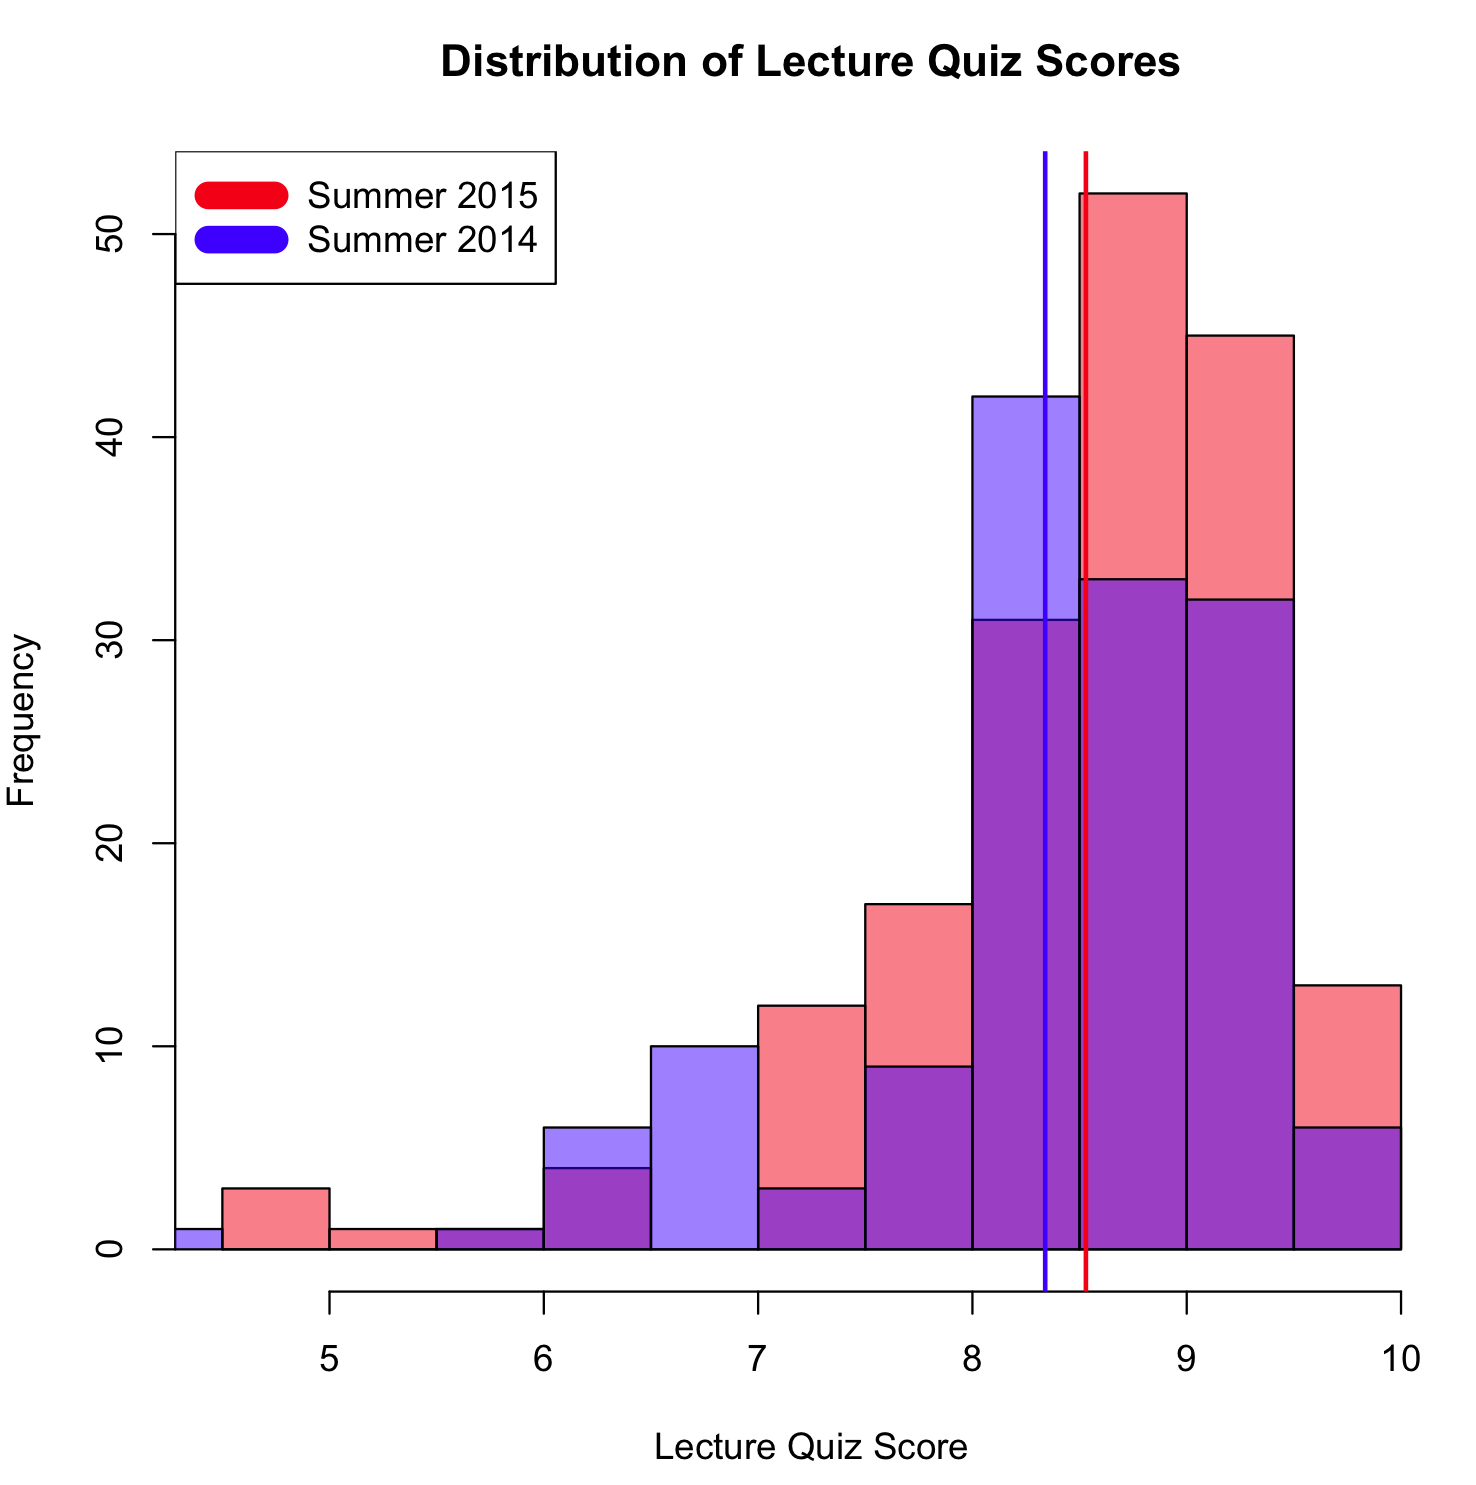
\includegraphics[width=2in]{img/chapter4/lq_su15_vs_su14}
\end{figure}
\end{column}
\begin{column}{2in}
\begin{scriptsize}
\begin{table}
  \begin{tabular}{|l|l|}
    \hline
    \textbf{Statistic} & \textbf{Value} \\
	\hline
	$\mu$ - 2015 & 8.530 \\
	\hline
	$\mu$ - 2014 & 8.340 \\
	\hline
	$\sigma$ - 2015 & 0.955 \\
	\hline
	$\sigma$ - 2014 & 1.070 \\
	\hline
	Shapiro-Wilk - 2015 & p = 7.4e-11 \\
	\hline
	Shapiro-Wilk - 2014 & p = 3.55e-11 \\
	\hline
	Wilcoxon Signed-Rank & p = 0.0857 \\
	\hline
	Cohen's D & 0.188 \\
	\hline
  \end{tabular}
\end{table}
\end{scriptsize}
\end{column}
\end{columns}
\end{frame}

\begin{frame}{Fall 2014 (Distance Learning) vs. Summer 2015}
\begin{columns}
\begin{column}{2in}
\begin{figure}
	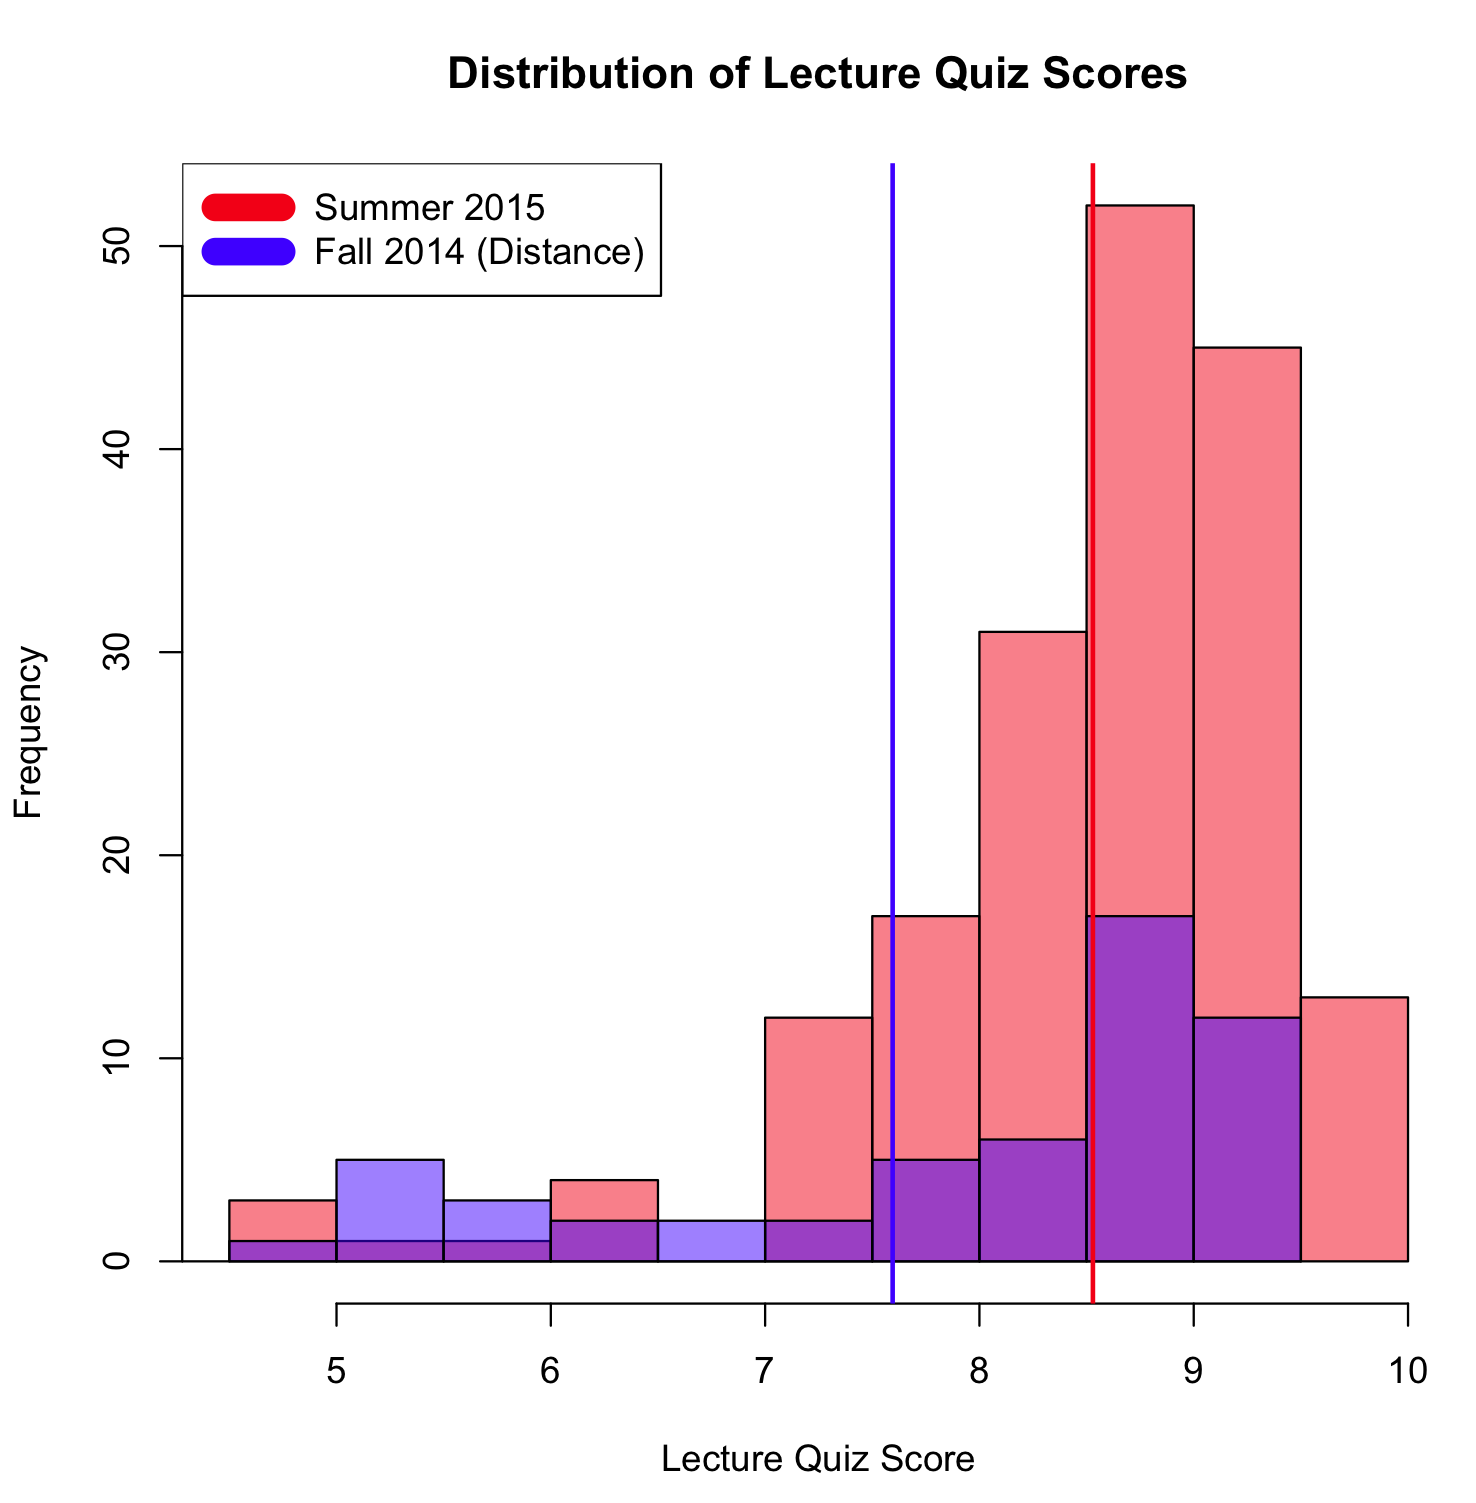
\includegraphics[width=2in]{img/chapter4/lq_su15_vs_f14d}
\end{figure}
\end{column}
\begin{column}{2in}
\begin{scriptsize}
\begin{table}
  \begin{tabular}{|l|l|}
    \hline
    \textbf{Statistic} & \textbf{Value} \\
	\hline
	$\mu$ - 2015 & 8.530 \\
	\hline
	$\mu$ - 2014 & 7.595 \\
	\hline
	$\sigma$ - 2015 & 0.955 \\
	\hline
	$\sigma$ - 2014 & 1.858 \\
	\hline
	Shapiro-Wilk - 2015 & p = 7.4e-11 \\
	\hline
	Shapiro-Wilk - 2014 & p = 7.746e-07 \\
	\hline
	Wilcoxon Signed-Rank & p = 0.001259 \\
	\hline
	Cohen's D & 0.754 \\
	\hline
  \end{tabular}
\end{table}
\end{scriptsize}
\end{column}
\end{columns}
\end{frame}

\begin{frame}{Spring 2015 (Distance Learning) vs. Summer 2015}
\begin{columns}
\begin{column}{2in}
\begin{figure}
	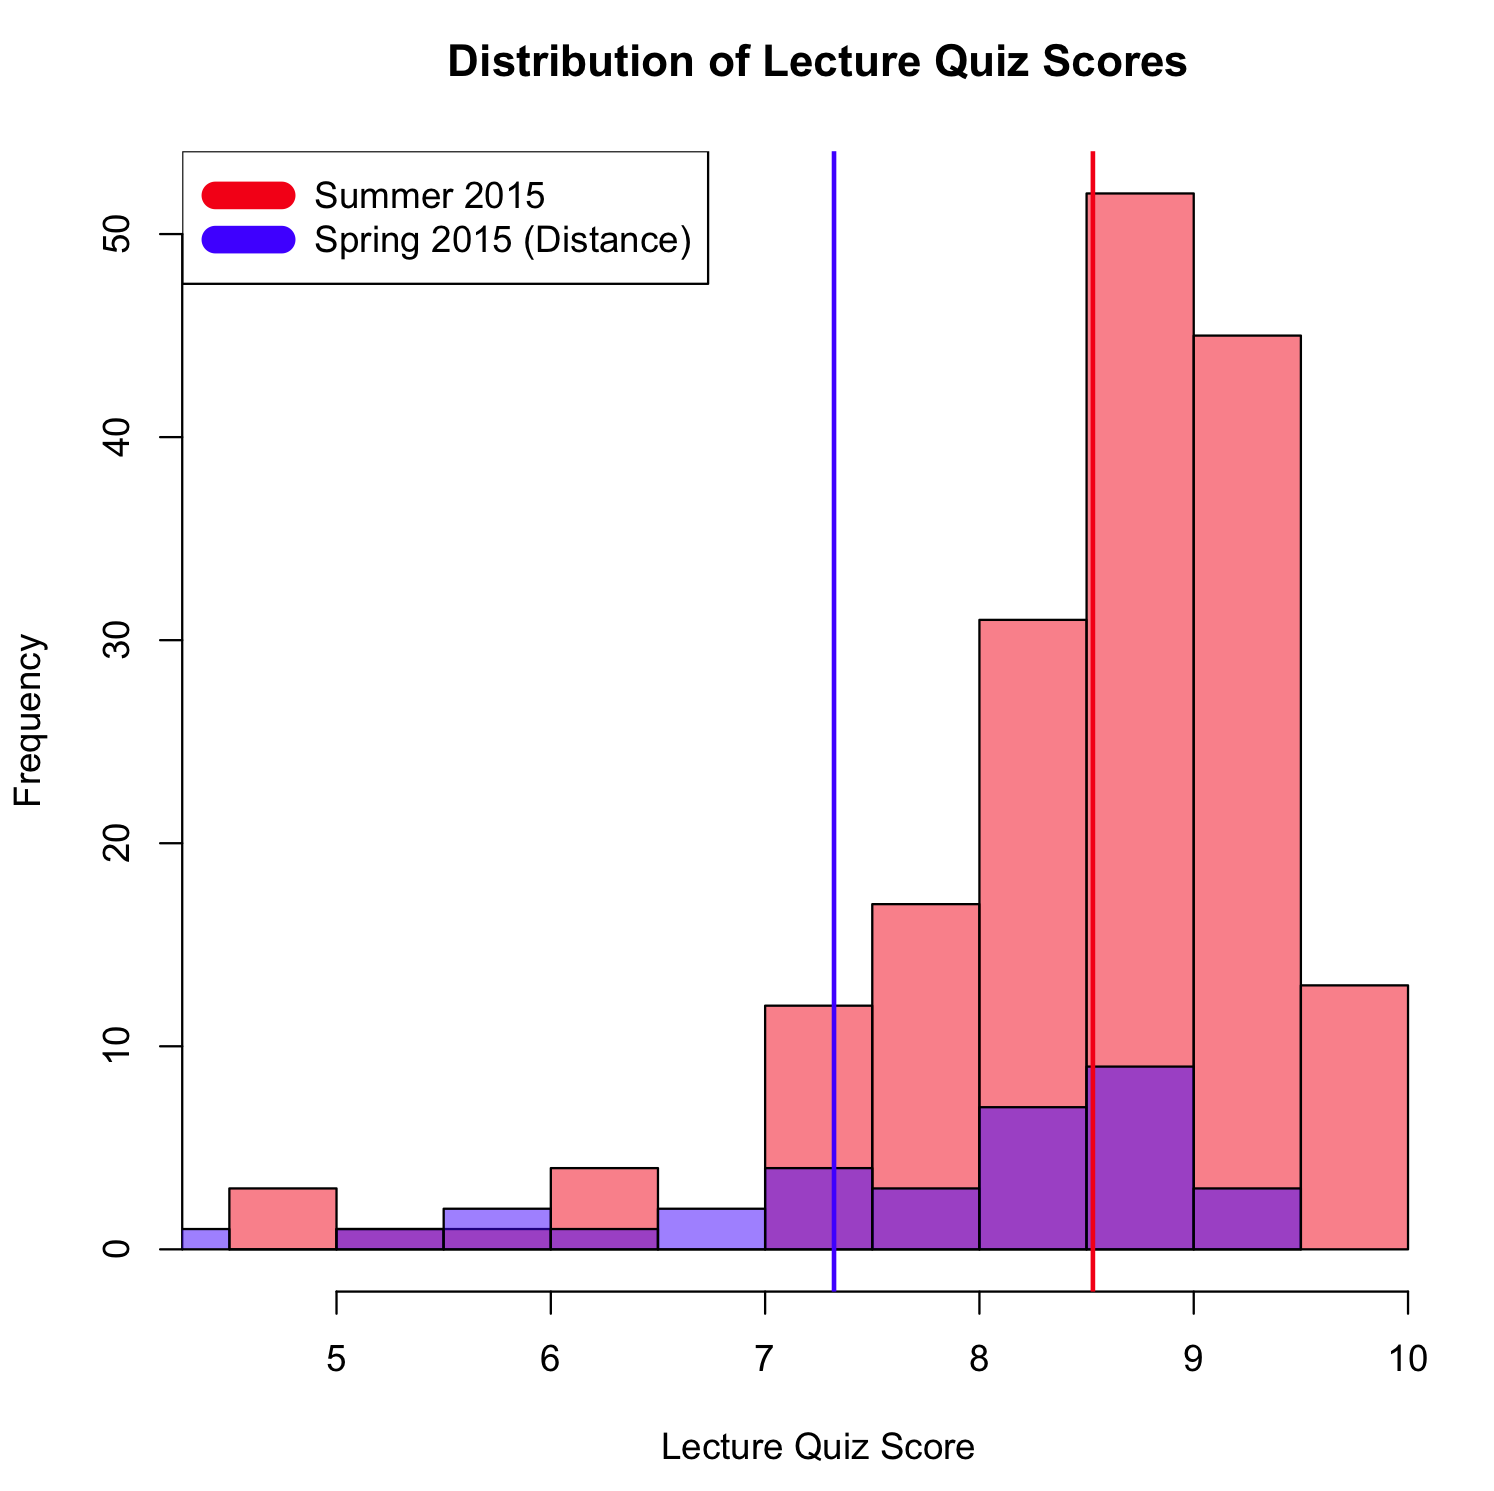
\includegraphics[width=2in]{img/chapter4/lq_su15_vs_sp15d}
\end{figure}
\end{column}
\begin{column}{2in}
\begin{scriptsize}
\begin{table}
  \begin{tabular}{|l|l|}
    \hline
    \textbf{Statistic} & \textbf{Value} \\
	\hline
	$\mu$ - Su 2015 & 8.530 \\
	\hline
	$\mu$ - Sp 2015 & 7.321 \\
	\hline
	$\sigma$ - Su 2015 & 0.955 \\
	\hline
	$\sigma$ - Sp 2015 & 1.885 \\
	\hline
	Shapiro-Wilk - Su 2015 & p = 7.4e-11 \\
	\hline
	Shapiro-Wilk - Sp 2015 & p = 9.398e-05 \\
	\hline
	Wilcoxon Signed-Rank & p = 3.185e-05 \\
	\hline
	Cohen's D & 1.037 \\
	\hline
  \end{tabular}
\end{table}
\end{scriptsize}
\end{column}
\end{columns}
\end{frame}

\begin{frame}{Trends with Lecture Quiz Scores}
  \begin{itemize}
    \item Summer 2015 lecture quiz scores are consistently higher than those in previous semesters.
    \item The effect size of these scores is also very high (especially against spring 2015).
    \item I did not expect this result - more testing is needed to see if it carries through in future semesters.
  \end{itemize}
\end{frame}

%%%%%%%%%%%%%%%%%%
% Conclusions and Future Work %
%%%%%%%%%%%%%%%%%%
\subsection*{Conclusions and Future Work}

\begin{frame}{Conclusions}
  \begin{enumerate}
    \item My preliminary analysis of CITA is quite promising - scores on the homework, quizzes, and BEMA either stayed the same or increased.
    \item Online sections of the class seem to show the most improvement with the addition of the CITA scaffolding.
    \item It will be especially interesting to conduct the analysis with the multi-step problem.
  \end{enumerate}
  \begin{center}
  We are off to a great start!
  \end{center}
\end{frame}

\begin{frame}{Future Work}
  \begin{enumerate}
    \item IRB Approval for the Study
    \item Iterative Development of the System
    \item Qualitative and Quantitative Analysis of the Results
  \end{enumerate}
  \begin{center}
  One day, I would love to pass the torch to another researcher!
  \end{center}
\end{frame}

\begin{frame}{}
  \begin{center}
  Thank You for Your Attention!
  \end{center}
\end{frame}

\subsection*{Extra Slides}

\begin{frame}{Enrollment in Electricity and Optics}
  \begin{figure}
    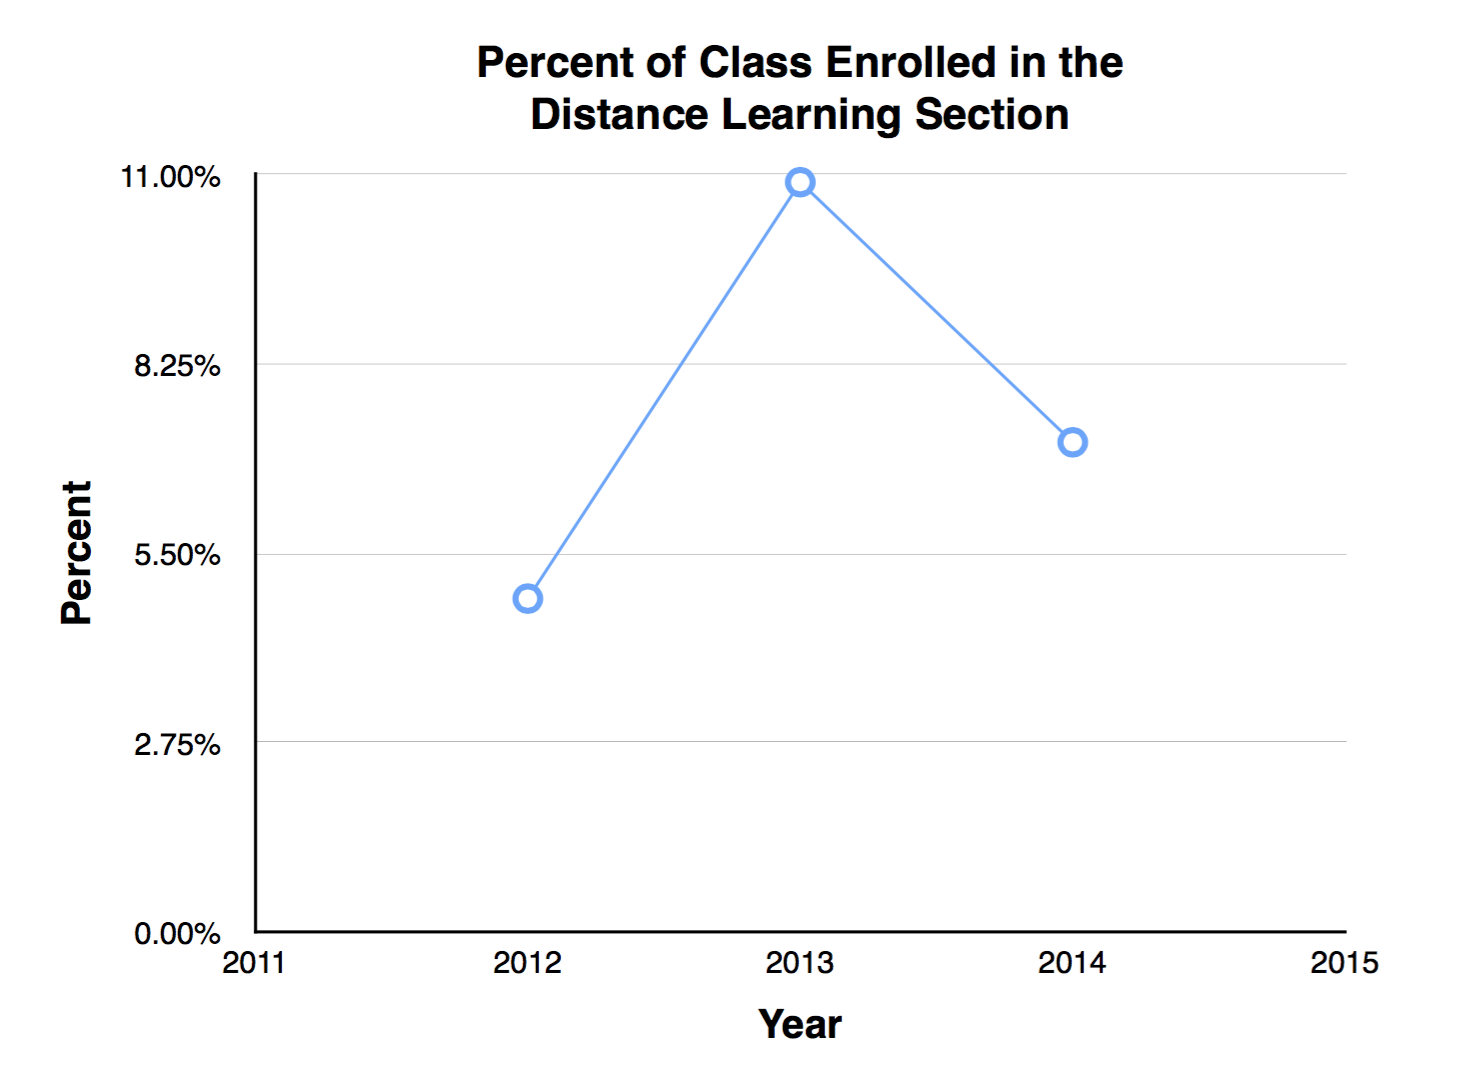
\includegraphics[width=3.5in]{img/chapter1/percent}
  \end{figure}
\end{frame}

\end{document}


